\section{Introduction}
Code translation typically refers to translating code from one programming language to another while preserving the functionality of the source code~\cite{pan2024lost,sun2024survey,eniser2024towards,dou2024s}. It has broad applications, including refactoring code written in outdated languages~\cite{aggarwal2015using}, transitioning from simple but slow languages to more complex and faster ones~\cite{szafraniec2022code}, enabling multi-platform project migration~\cite{nguyen2013lexical,nguyen2014migrating}, and addressing data scarcity issues through synthetic data generation~\cite{ren2020codebleu}. Automatic code translation can significantly reduce effort, which is why it has garnered widespread attention in recent years~\cite{bahdanau2014neural, chen2018tree, artetxe2018unsupervised, devlin2018bert, feng2020codebert, guo2020graphcodebert, ahmad2021unified, guo2022unixcoder, zheng2023codegeex}. Numerous studies focus on code translation, and with the rise of large language models (LLMs), researchers have started applying them to code translation with promising results~\cite{yang2024exploring,lano2024using,nitin2024spectra}. 

To facilitate and fairly evaluate code translation performance\hy{revise English}, various benchmarks are introduced to assess different translation frameworks. Many crafted datasets like CodeNet~\cite{puri2021codenet}, Avatar~\cite{ahmad2021avatar}, and EvalPlus~\cite{liu2024your} are used for evaluation\hy{there are some other datasets around 2010-2014, including paired projects and automatically mined ones}, typically focusing on simple tasks at the snippet or function level. This limitation mainly stems from earlier model-based methods' restricted window lengths~\cite{feng2020codebert,guo2020graphcodebert,ahmad2021unified,guo2022unixcoder}. In recent years, some benchmarks start extracting snippets or files from real-world projects for evaluation~\cite{yan2023codescope,yan2023codetransocean}. However, these benchmarks still fall short of addressing real-world development needs~\cite{pan2024lost}, where we often need to migrate entire code repositories rather than just a snippet, function, or a single file. 

To fill this gap, we introduce a repository-level code translation benchmark named RepoTransBench. Unlike previous benchmarks, RepoTransBench operates at the repository level, translating entire repositories from one language to another. We collect real-world repositories from the-stack~\cite{the-stack} and the-stack-v2~\cite{the-stack-v2} to construct this benchmark\hy{brielfy describe what they are}. We filter repositories based on their star count and language composition, then check for conditions such as cross-file dependencies, test cases included, and whether be successfully executed\hy{revise English}. Ultimately, we select candidate repositories that meet the criteria. With the help of LLM assistants~\cite{openai2023gpt4,Claude,deepseekv2}\hy{what does LLM assistant do?}, we manually translate the test cases of these repositories into the target language and provide corresponding executable test suites.

As shown in Table.~\ref{table:datasets}, RepoTransBench is compared with previous well-known code translation benchmarks. RepoTransBench is repository-level in terms of granularity which has 10x tokens and lines than previous benchmarks and more complex dependency to understand\hy{revise english}. Moreover, RepoTransBench requires translators to correctly configure config files and address the complex interfaces involved in repository translation\hy{not clear}.

We evaluate state-of-the-art LLMs~\cite{openai2023gpt4,Claude,deepseekv2,llama3} on RepoTransBench, and the results show that even the best-performing model, Claude-3.5-Sonnet, achieves only a 7\% average full execution success rate and the pass@3 is just 12\%. Meanwhile, smaller open-source models like Llama-3.1-8B-Instruct have a pass@3 rate of 0\%, indicating that repository-level code translation is nearly impossible for users with limited resources.\hy{how do you evaluate pass or fail?}

To further explore the potential of LLMs for repository-level translation, we adopt an iterative debugging approach, feeding error-related information back into the LLMs~\cite{pan2024lost}. After five iterations, GPT-4o achieves an average full execution success rate of 20\% and a pass@3 of 33\%. However, these results are still relatively low, leaving much room for research into efficient and high-performing repository-level code translation.

Our main contributions are:

\begin{itemize}[left=10pt]
    \item We introduce the first real-world repository-level code translation benchmark named \textbf{RepoTransBench} based on automatic executable evaluation, which has more than x10 tokens and more complex dependency.
    \item We comprehensively evaluate both open-source and closed source state-of-the-art models, revealing that current LLMs struggle to achieve repository-level translation.
    \item To explore the potential of LLMs in repository-level translation, we iteratively feed error-related information back to LLMs and observe a significant improvement.\hy{can revise the sentence}
    \item We conduct a detailed error analysis to provide insights for further improvements in repository-level code translation.
\end{itemize}


\begin{table}[t]
  \centering
  \footnotesize
  \setlength\tabcolsep{1.5pt}
  \caption{Overview of existing code translation datasets. Considering the translation of Python to Java, we report the number of samples and the average number of tokens, lines, functions, classes, and import statements per sample of each task. \#Tokens counts are based on OpenAI’s tiktoken tokenizer (\url{https://github.com/openai/tiktoken}). \#Funcs, \#Classes and \#Imports counts are based on tree-sitter (\url{https://tree-sitter.github.io})}

% \vspace*{-10pt}
\resizebox{\columnwidth}{!}{
    \begin{tabular}{l|c|c|c|c|c|c|c|c|c|c|c}
    \hline
    \multicolumn{1}{c|}{\textbf{Dataset}} & \multicolumn{1}{c|}{\textbf{Year}} & \multicolumn{1}{c|}{\textbf{Type}} & \multicolumn{1}{c|}{\textbf{Level}} & \multicolumn{1}{c|}{\textbf{Config File}} & \multicolumn{1}{c|}{\textbf{Evaluation}} & \multicolumn{1}{c|}{\textbf{\#Samples}} & \multicolumn{1}{c|}{\textbf{\#Tokens}} & \multicolumn{1}{c|}{\textbf{\#Lines}} & \multicolumn{1}{c|}{\textbf{\#Funcs}} & \multicolumn{1}{c|}{\textbf{\#Classes}} & \multicolumn{1}{c}{\textbf{\#Imports}} \\
    \hline
    \hline
    CodeNet~\cite{puri2021codenet} & 2021 & Crafted & Snippet & Not Req & Auto, Execution & 200 & 99 & 12 & 1 & 0 & 0 \\
    \hline
    Avatar~\cite{ahmad2021avatar} & 2021 & Crafted & Snippet & Not Req & Auto, Execution & 250 & 175 & 18 & 1 & 0 & 1 \\
    \hline
    EvalPlus~\cite{liu2024your} & 2023 & Crafted & Function & Not Req & Auto, Execution & 164 & 64 & 6 & 1 & 0 & 0 \\
    \hline
    CodeScope~\cite{yan2023codescope} & 2023 & Real-World & Snippet & Not Req & Auto, Execution & 30 & 259 & 28 & 1 & 0 & 1 \\
    \hline
    CodeTransOcean~\cite{yan2023codetransocean} & 2023 & Real-World & File & Not Req & Auto, Similarity & 1029 & 253 & 24 & 2 & 0 & 1 \\
    \hline
    \hline
    \rowcolor{gray!20} % 设置灰色的行
    % RepoTransBench & 2024 & Python2Java & Real-World & Repository & Auto, Execution & 100 & Yes & 3431 & 352 & 34 & 5 & 12 \\
    \textbf{RepoTransBench} & \textbf{2024} & \textbf{Real-World} & \textbf{Repository} & \textbf{Require} & \textbf{Auto, Execution} & \textbf{100} & \textbf{3431} & \textbf{352} & \textbf{34} & \textbf{5} & \textbf{12} \\
    \hline
    \end{tabular}}%
 \label{table:datasets}
% \vspace*{-2em}
\end{table}%
% 代码翻译通常是指将一种语言的代码翻译成另一种语言的代码，同时保留源语言代码的功能。代码翻译的应用场景十分广泛，他可以用于对过时的语言编写的代码进行重构、用于将简单但速度慢的语言切换到复杂但速度快的语言、用于多平台的项目迁移、此外还可用于合成数据以应对当前面临的数据匮乏等问题。自动代码翻译能够很大程度地减少effort，因此近年来受到广泛的关注。许多工作针对代码翻译进行了研究，随着LLMs的普及，Researcher也尝试将LLMs应用到代码翻译中来并取得了不错的效果。为了方便和公平地评测代码翻译的效果，许多benchmark被提出，用于评估各种代码翻译框架的性能。许多crafted的数据集比如CodeNet、Avatar、evalplus被提出用于评测，他们通常是snippet或者function level的简单任务。这通常是因为早年间受限于model-based 方法有限的窗口长度。近年来也有一些benchmark从real-world的Project中抽取snippet或者file用于评估。然而，这些benchmark并不真的符合真实开发场景的需要，在真实的开发场景中，我们往往需要对整个code repository进行迁移，而非code snippet、a single function or file。to fill in this gap，我们提出了一个repository-level的代码翻译benchmark，名为RepoTransBench。与先前的benchmark不同的是，名为RepoTransBench是以仓库为粒度，将整个仓库从一种语言翻译成另一种语言。我们从the stack 和 the stack v2两个数据集中获取来自真实世界的repository用于构建benchmark。我们使用repository的stars数、language占比对repository进行过滤，随后检查repository是否存在跨文件依赖、是否自带testcase以及是否能够成功执行等条件等等，最终筛选出来符合要求的Candidate repository。如表1所示，我们将RepoTransBench和先前知名的代码翻译benchmark进行对比，在粒度上RepoTransBench是repository-level，此外，相比于先前level的benchmark，RepoTransBench要求translator能够正确配置config文件，以应对repository翻译时需要调用的复杂接口的问题。我们在LLM assistant的帮助下，人工将这些repository的testcase翻译成目标语言的testcase，并提供相应的可执行的测试套件。我们对当前的benchmark进行统计后，发现RepoTransBench在复杂度上明显强于现有的benchmark。在平均token和line数量上，RepoTransBench是file级别的codetransocean十倍以上。除了长度以外，复杂的infile、crossfile的调用关系也是代码翻译的难点之一，RepoTransBench的平均func数达到了34，平均的class数达到了5，而目前最复杂的benchmark却分别平均只有2两个func，几乎没有class。此外，repository-level 代码翻译的一个突出难点在于其复杂的crossfile调用关系，我们统计了import statement的数量，平均每个repository有12个import语句，相对而言，现有的其他的benchmark平均只有不到一个import statement。我们使用最先进的LLMs在RepoTransBench进行评测，结果发现，表现最好的claude-3.5-Sonnet平均一次通过的可能性只有7%，pass@3也仅仅只有12%。而开源大模型中参数量较小的Llama-3.1-8B-Instruct的pass@3竟然为0，说明对于有限资源的用户来说，进行repository-level的代码翻译几乎不可能。为了进一步探究LLMs进行repository level翻译的可能，我们采用迭代debug的方式，将error-related信息反馈给LLMs，在迭代五轮之后，GPT-4o的平均完全执行通过率达到了20%，pass@3达到了33%，然而这依旧处于一个相当低的水平，留下了值得探究的高效的高性能的repository-level代码翻译的问题。
% Our main contributions are:
% 我们首次提出了一个基于自动可执行评估的real-world的仓库级别的代码翻译benchmark
% 我们对目前最先进的开源、闭源模型进行了评测详尽的评测，发现目前的LLMs很难一次就成功完成仓库级别的代码翻译任务
% 为了进一步探究LLMs在仓库级别代码翻译上的可能性，我们将error-related 信息反馈给模型，通过迭代debug，发现能够显著提高翻译的完全通过率。
% 我们对错误进行了详尽的分析，为进一步提升仓库级别代码翻译性能提供了参考



% 先前的代码翻译benchmark的翻译粒度只有function或者snippet或者file粒度的，这往往是因为受限于model-based 方法有限的窗口长度。随着LLMs的出现，他们支持更长的窗口长度，一些模型的窗口长度甚至拓展到128k、200k，这使得LLMs能够接受更多的信息，让整个代码仓库的翻译成为了可能。
% lost in translation研究了两个repo（cli、）翻译的结果，然而由于缺乏testcase，因此需要人工去分析翻译结果的正确性，这样难以拓展到大规模数据的评测上。
% 画一张图，上面三个小图表示片段、函数、file代码，下面一张是仓库代码包括一个tree和一些文件



\section{Background}
\subsection{Code Translation}
% 代码翻译通常是指将一种语言的代码翻译成另一种语言的代码，同时保留源语言代码的功能。代码翻译的应用场景十分广泛，他可以用于对过时的语言编写的代码进行重构、用于将简单但速度慢的语言切换到复杂但速度快的语言、用于多平台的项目迁移、此外还可用于合成数据以应对当前面临的数据匮乏等问题。自动代码翻译能够很大程度地减少effort，因此近年来受到广泛的关注。许多工作针对代码翻译进行了研究，随着LLMs的普及，Researcher也尝试将LLMs应用到代码翻译中来并取得了不错的效果。
Code translation involves converting source code written in one programming language into another language while preserving the original program's functionality and logic~\cite{pan2024lost,sun2024survey,eniser2024towards,dou2024s}. This process is essential in software engineering for several reasons, such as migrating legacy systems to modern languages~\cite{nguyen2013lexical,nguyen2014migrating}, improving code performance by translating to more efficient languages~\cite{aggarwal2015using}, and enabling cross-platform compatibility~\cite{szafraniec2022code}. As programming languages continue to evolve, the demand for accurate and efficient code translation techniques has grown, making it a critical area of research and development~\cite{bahdanau2014neural, chen2018tree, artetxe2018unsupervised, devlin2018bert, feng2020codebert, guo2020graphcodebert, ahmad2021unified, guo2022unixcoder, zheng2023codegeex}. Many studies focus on code translation, which can be broadly divided into two main categories: non-LLM-based and LLM-based approaches~\cite{pan2024lost}. Existing non-LLM-based code translation techniques can be categorized into several main groups. Parser-based tools like ANTLR~\cite{ANTLR} rely on manually defined grammar rules to translate source code between languages. Transpilers such as Babel~\cite{Babel}, Emscripten~\cite{Emscripten}, JSweet~\cite{JSweet}, and GWT~\cite{GWT} convert source code from one language to another, often used to ensure compatibility across platforms or systems. Domain-specific translators like CxGo~\cite{CxGo}, C2Rust~\cite{c2rust}, and JavaToCSharp~\cite{javaTocsharp} focus on specific language pairs, offering targeted translation solutions. Intermediate language compilers like Haxe~\cite{Haxe} compile code to a variety of target languages by using an intermediate format. Interface generators such as SWIG~\cite{SWIG} create cross-language bindings, allowing different languages to interact with each other without direct code translation. LLM-based approaches leverage large language models to automatically translate code between programming languages. Prominent models in this category include StarCoder~\cite{li2023starcoder,lozhkov2024starcoder}, SantaCoder~\cite{allal2023santacoder}, CodeGen~\cite{nijkamp2022codegen}, CodeT5~\cite{wang2021codet5}, CodeX~\cite{chen2021evaluating}, and more latest models such as the Llama series (Llama, Llama2, Llama3...)~\cite{llama,llama2,llama3}, the ChatGPT series (GPT-3.5-turbo, GPT-4, GPT-4o...)~\cite{openai2023gpt4}, the DeepSeek series (DeepSeekCoder, DeepSeek-v2, DeepSeek-v2.5...)~\cite{deepseekv2}, and the Claude series (Claude-3.5-sonnet...)~\cite{Claude}. These models are trained on large codebases and have strong comprehension and instruction-following abilities, which can perform accurate and efficient code translations.


\hy{there are may other related work  around 2010-2014}


\hy{There is a related work DeepAM, which discussed the limitation of bilingual projects, as well as the automatic mining of API mappings to reduce manual effort in code migration: 
https://arxiv.org/pdf/1704.07734}

\subsection{Benchmarks for Code Translation}
Benchmarks provide standardized datasets and metrics that allow researchers and developers to compare different translation techniques objectively. As shown in Figure.~\ref{fig:TranslationLevel}, previous works such as CodeNet~\cite{puri2021codenet}, Avatar~\cite{ahmad2021avatar} and EvalPlus~\cite{liu2024your} typically focus on crafted translation tasks, which involve translating a code snippet or function into the target language. In recent years, some works have attempted to extract a snippet or a single file from real-world repositories for code translation, such as CodeScope~\cite{yan2023codescope} and CodeTransOcean~\cite{yan2023codetransocean}. Although these benchmarks can evaluate the capabilities of existing code translation techniques to some extent, they do not reflect the performance of current techniques on real-world code translation tasks. In real-world code translation tasks, it is often necessary to translate an entire repository. Such tasks typically involve translating longer and more complex code repositories. On one hand, this requires ensuring that the techniques can handle sufficiently long code contexts, and on the other hand, it also requires the techniques to understand complex in-file and cross-file dependencies, which makes the translation more challenging. Previous work~\cite{pan2024lost} manually studies two open-source projects (Apache Commons CLI~\cite{apachecommonscli} and py Click~\cite{click}) and finds that current LLMs struggle to complete the translation tasks of entire projects. However, they do not provide a sufficient number of repositories and corresponding automatic test suites for evaluation. To this end, we propose the first repository-level code translation benchmark, along with corresponding automatic test suites, providing an evaluation standard for whole-repository code translation.


\begin{figure}
    \centering
    % \vspace{-10pt}
    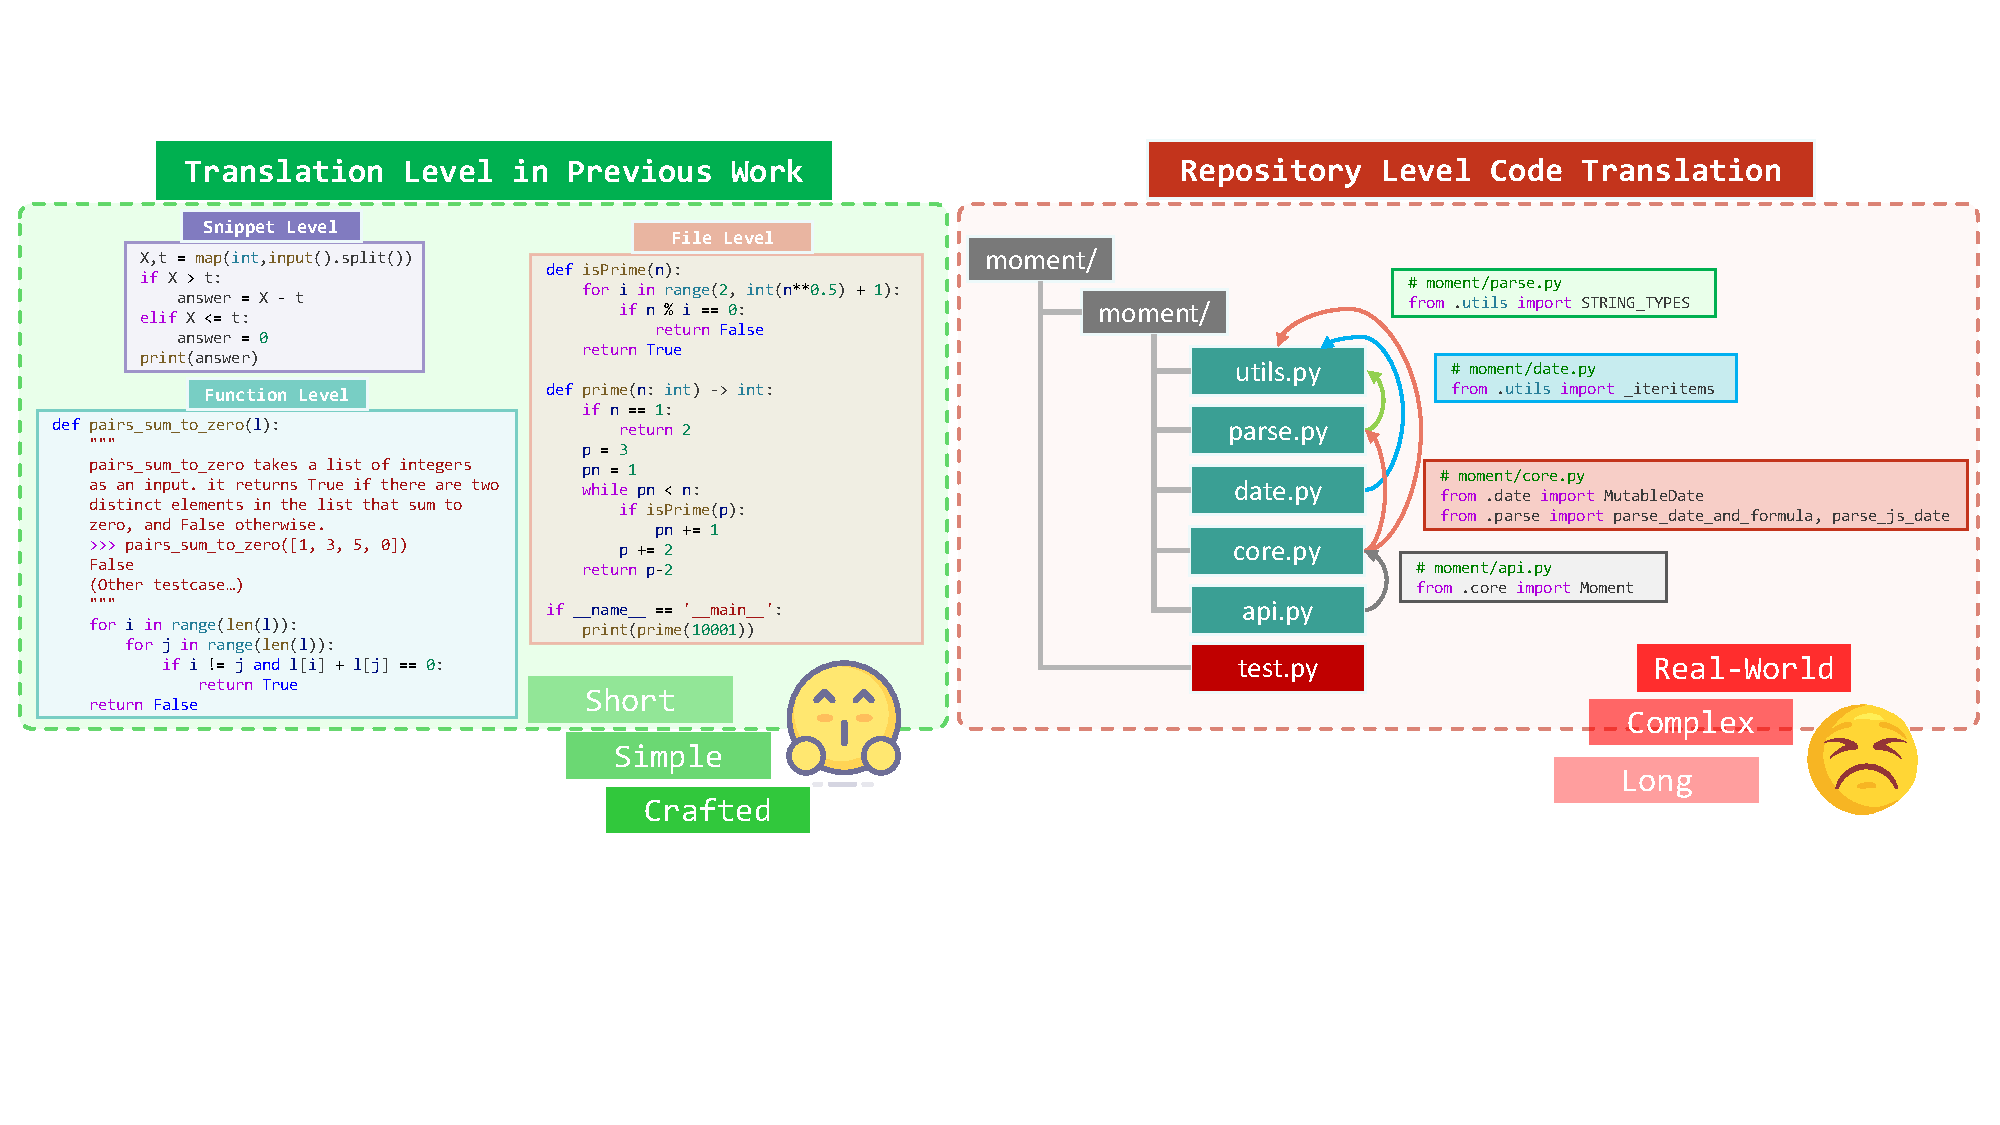
\includegraphics[width=\linewidth]{figures/TranslationLevel.pdf}
    % \vspace{-1em}
    \caption{Comparison of Translation Level.}
   % \vspace{-0.5em}
    \label{fig:TranslationLevel}
\end{figure}



\section{RepoTransBench}

In this section, we introduce RepoTransBench. The construction process of RepoTransBench includes three phases: task definition, data collection, and test case construction.

\subsection{Task Definition}
Repository-level code translation aims to translate the entire repository from one language to another. Due to the limited context window and performance of non-LLM techniques~\cite{pan2024lost}, we use LLMs to achieve the translation tasks.

\subsubsection{Language Selection}
Referring to the \texttt{TIOBE index}~\cite{TIOBE-Index} for language popularity, we select Python, C++, Java, C, and C\# as candidate languages. Considering Python is popular for its simplicity, ease of use, and rapid prototyping, but has low execution efficiency, while Java, on the other hand, is favored for enterprise-level applications, offering better performance, stability, and faster execution~\cite{szafraniec2022code}, we choose Python as the source language and Java as the target language. 

\subsubsection{Metric Selection}
Previous snippet or function-level code translation tasks usually involve shorter code, which can easily generate test cases using LLMs~\cite{puri2021codenet,ahmad2021avatar,liu2024your,yan2023codetransocean}. For file-level code translation tasks, as shown in Table~\ref{table:datasets}, CodeTransOcean~\cite{yan2023codescope} uses a similarity-based metric for evaluation. However, for repository-level code translation, \textbf{syntactic correctness} and \textbf{functional correctness} are more important~\cite{pan2024lost}. 
\begin{itemize}[left=10pt]
    \item Repositories with high similarity may still fail to compile or fail to achieve the expected functionality.
    \item Repositories that implement the same functionality can have vastly different code structures, leading to low similarity.
\end{itemize}
These reasons make similarity-based metrics a poor evaluation method to evaluate the performance of repository-level code translation. Therefore, we decide to use execution-based methods as the evaluation metric. 

\subsubsection{Issues Identification}
In fact, obtaining test cases for the entire repository in the target language is not easy. We have identified the following reasons:
\begin{itemize}[left=10pt]
    \item \textbf{Long Context Issue:} The test cases in repositories are often very long, with a substantial number of assert statements. Relying solely on LLMs makes it difficult to translate them accurately.
    \item \textbf{Language Feature Issue:} For example, it's quite common to have multiple classes in a single Python file, and global variables and functions can be defined directly in the file without being enclosed in a class. However, in Java, classes are usually placed in separate files, and all properties and functions need to be wrapped within a class.
    \item \textbf{Path Issue:} If the file structure is not standardized, the paths in different files of a Python repository may differ significantly from those in a Java repository. This makes it challenging to correctly handle paths in test cases during translation.
\end{itemize}

\subsubsection{Standard Statement}
In previous function-level code translation tasks, we expect a Python function to be translated into a Java function wrapped in a class. However, translating all functions in a Python repository into individual Java classes and combining them to form the entire Java repository is clearly not in line with the style of a real Java repository. To better define repository-level code translation, we manually examine over 50 repositories to understand the style and characteristics of real-world repositories, and ultimately, we establish the following translation standards for our benchmark with a live example shown in Figure.~\ref{fig:Python2Java}.
\begin{itemize}[left=10pt]
    \item We use the popular Java framework Maven~\cite{maven} as the standard framework for target Java repositories. We expect functional code to reside in the \texttt{src/main/java} directory and test code to reside in the \texttt{src/test/java} directory. Resource files in Python can exist anywhere, but we expect them to be located in the \texttt{src/main/resources} or \texttt{src/test/resources} directories in the target Java repository.
    \item Unlike previous function-level code translation tasks, we treat a Python file containing multiple functions as a single Java class, rather than wrapping each Python function into its own class. If there are multiple classes in one Python file, these classes will correspond to individual Java class files.
    \item For issues related to language differences, such as private attribute access, Python does not have visibility modifiers, and class attributes can be accessed directly via \texttt{object.attribute}. However, in Java, class attributes are often marked with the \texttt{private} modifier and accessed or modified through \texttt{get} and \texttt{set} methods. For such issues, we ensure that the test cases meet the characteristics of the target language (Java) through manual checks during the construction of test cases, rather than serving as “next code token” predictors~\cite{pan2024lost}.
    \item Similar to function-level code translation~\cite{liu2024your}, when performing repository-level code translation, we also need to provide corresponding test cases in the target language as a reference, so the model understands the input and output formats. Additionally, we need to provide a reference project tree to clarify the expected structure of the target project for the LLMs.
\end{itemize}

\begin{figure}
    \centering
    % \vspace{-10pt}
    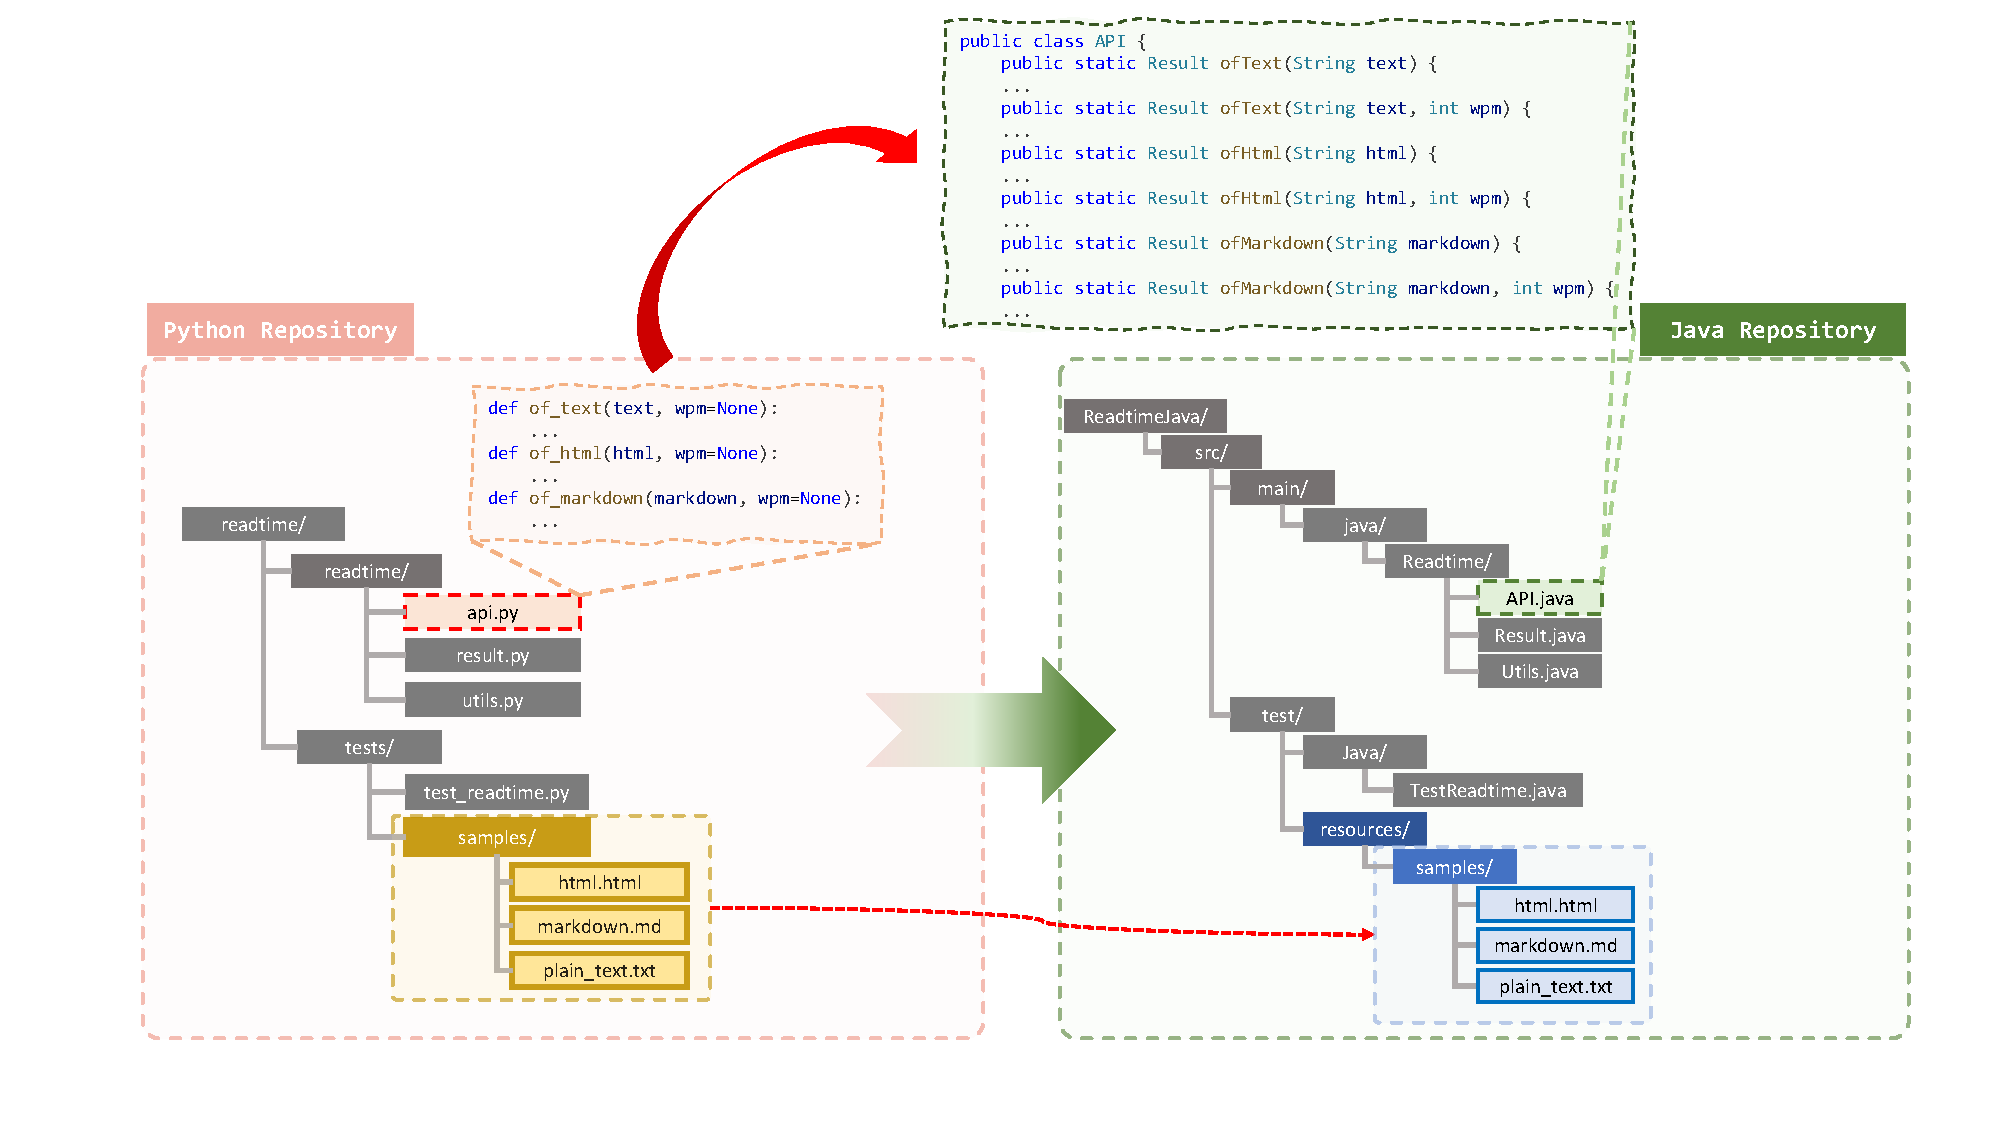
\includegraphics[width=\linewidth]{figures/Python2Java.pdf}
    % \vspace{-1em}
    \caption{Overview of the translation process.}
   % \vspace{-0.5em}
    \label{fig:Python2Java}
\end{figure}

\subsection{Data Collection}
The data collection process is illustrated in Figure~\ref{fig:DataCollection}. We use the training data of \texttt{Starcoder}~\cite{li2023starcoder,lozhkov2024starcoder} series models, \texttt{the-stack}~\cite{the-stack} and \texttt{the-stack-v2}~\cite{the-stack-v2}, as our data sources. By filtering based on language and star count, we obtain the \texttt{Raw Repo List}. Then, by requesting the \texttt{GitHub REST API}~\cite{github-rest-api}, we redirect repositories that are forks of other repositories to their origin repositories. Additionally, we update information such as the star count in this list. We further filter the list based on language, size, and other criteria to obtain the \texttt{Updated Repository List}. Next, we download the repositories from the list and perform further filtering. We analyze the dependencies of the repositories with \texttt{tree-sitter}~\cite{tree-sitter} to ensure sufficient in-file and cross-file dependencies. Besides, we ensure that the test cases are existing, high-coverage and executable. Ultimately, we obtain our \texttt{Candidate Repository} for further processing.

% 数据收集流程如图fig:DataCollection所示，我们使用Starcoder系列模型的训练数据the stack and the stack v2作为我们的数据来源，根据语言和star数进行filtering，得到raw repo list，随后我们通过请求github api，对于fork自其他repository的repository我们重定向到Origin repository，此外我们更新这个list中的star等信息，然后再使用语言、size等标准过滤得到updated repository list，然后我们将list中的repository下载下来，对其进行进一步的过滤，采用tree-sitter进行依赖解析的获取repository的依赖情况，确保repository的testcase存在并可执行通过，最终得到我们的Candidate repository

\begin{figure}
    \centering
    % \vspace{-10pt}
    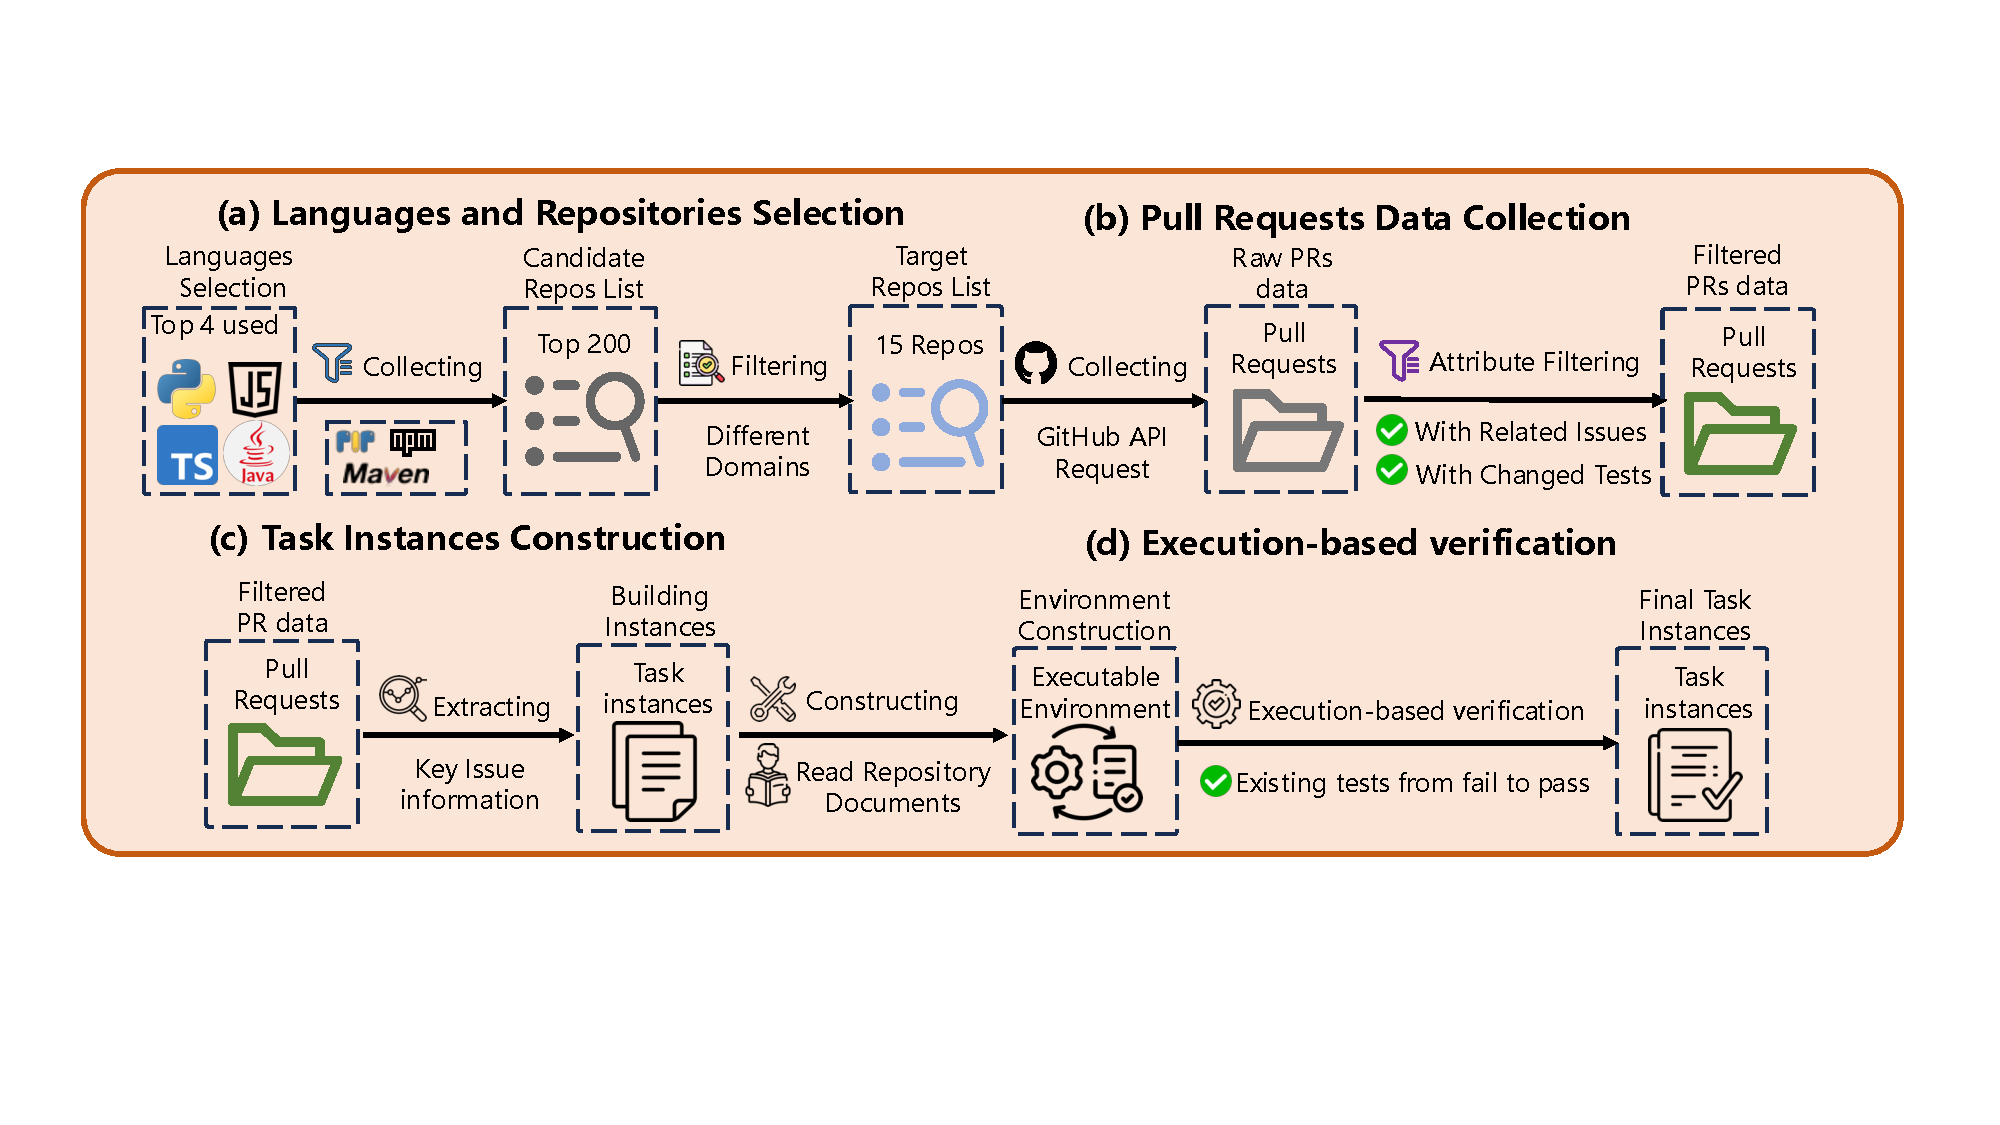
\includegraphics[width=\linewidth]{figures/DataCollection.pdf}
    % \vspace{-1em}
    \caption{Overview of Data Collection.\hy{revise "Test Case Existing"}}
   % \vspace{-0.5em}
    \label{fig:DataCollection}
\end{figure}

\subsubsection{Initial Filtering of Repository List} \label{sec:Initial}

For the data source, we choose to use \texttt{the-stack} and \texttt{the-stack-v2} as our data sources. We download the Python portion information of \texttt{the-stack} and \texttt{the-stack-v2} from Hugging Face~\cite{Hugging-Face} and group the information by repository name (using \texttt{max\_stars\_repo\_name} for \texttt{the-stack} and \texttt{repo\_name} for \texttt{the-stack-v2}). To ensure the credibility of the repositories, we prioritize repositories with a higher star count. We use the number of stars for filtering and retain only repositories with at least 10 stars. It is worth noting that the star counts are outdated, and many repositories are forks of others, which results in the actual star count being lower. This phenomenon is particularly pronounced in \texttt{the-stack}. Here, we use the star count only as an initial filter, and it does not represent the final selection criteria. After filtering, we obtain a \texttt{Raw Repo List}.

% 对于数据的来源，我们选择采用the stack and the stack v2 作为数据来源。参考TIOBE index中语言的流行度，我们将Python, C++, Java, C, C# 作为候选语言。考虑到Python is popular for its simplicity, ease of use, rapid prototyping 但是执行效率低. Java, on the other hand, is favored for enterprise-level applications, offering performance, stability, and faster. 因此在语言的选择，我们使用Python作为源语言，目标语言选择为Java。我们从huggingface上下载下来the stack 和the stack v2 的Python部分的数据，按照repository的名称对数据进行分组（max_stars_repo_name for the stack and repo_name for the stack v2）。为了保证repository的可信度，我们优先选择使用star数高的repo，我们使用star数量进行filtering，只保留star数量不低于10的repository，值得注意的是，这里的star数量已经过时了，并且很多repo都是fork自其他repo，所以真实的star数偏低，这在the stack上表现尤为明显，我们在这里仅仅是作为初筛，这个star数并不代表最终的筛选。经过筛选，我们最终得到一个信息并非完全准确的Raw Repo List。

\subsubsection{Repository List Updating}

After obtaining the \texttt{Raw Repo List}, we update the repository information by calling the \texttt{GitHub REST API}~\cite{github-rest-api} and perform further filtering. We check whether a repository exists, removing projects that do not exist. Besides, some projects are forked from other repositories, in which case we redirect to the origin repository and use the original repository information as the standard.

We also find that although we filter the data from the Python dataset in Section~\ref{sec:Initial}, many repositories have a primary language other than Python. To ensure we obtain a Python project, we require the percentage of Python language to be the largest among all languages, excluding frontend languages (e.g., HTML, CSS, etc.).

We then use the star count for further filtering, retaining only repositories with more than 50 stars. To reduce storage pressure, we keep only repositories with a size below 1024 KB. Finally, we obtain the cleaned \texttt{Updated Repo List}.

% 我们在得到Raw Repo List之后，通过调用github的api更新repository的信息并进行进一步的filtering。我们通过请求info api判断repository是否存在，剔除掉不存在Project。有些Project是fork自其他repo，如果是的话就是重定向到Origin repo，并以Origin repo的信息为准。随后我们发现，尽管我们是从the stack 的python数据集部分筛选出来的数据，很多repository含量最高的language却不是python，为了保证我们能够得到一个python的project，我们要求python的size在除了前端语言(html,css..)之外所有语言中占比最高。随后我们使用star数进行filtering，只保留star数高于50的，为了减少存储压力，我们只保留size在1024以下的repository。最终我们得到清洗过后的Updated repo list

\subsubsection{Repository Downloading}

We clone the raw repositories from the \texttt{Updated Repo List} to the local environment for subsequent analysis and filtering.

% 我们将Updated repo list中的repository clone到本地中来，用于后续的分析和filtering。

\subsubsection{Filtering for Raw Repository}

For repository-level code, a prominent feature is the existence of in-file and cross-file dependencies. To ensure that a sufficient number of repositories contain in-file and cross-file dependencies rather than just isolated snippets or functions, we use the popular multi-language tool \texttt{tree-sitter} to perform dependency parsing on the repositories, capturing functions, classes, and import statements and identifying the in-file and cross-file dependencies.

It is important to note that our benchmark aims to construct a translation dataset for individual repositories. However, thanks to Python's excellent ecosystem, it includes many convenient third-party packages, like \texttt{pytorch}~\cite{pytorch}, \texttt{tensorflow}~\cite{tensorflow}, etc. In fact, we often do not have the need to translate such repositories into other languages. We conduct a preliminary study on around one hundred repositories and obtain a blacklist. If a repository contains any packages from the blacklist, it will not be considered. Examples of packages on the blacklist include deep learning libraries like \texttt{pytorch}~\cite{pytorch}, \texttt{tensorflow}~\cite{tensorflow}, and \texttt{nltk}~\cite{nltk}, etc, data science libraries like \texttt{scikit-learn}~\cite{scikit-learn} and \texttt{jupyter-notebook}~\cite{jupyter}, etc, and data visualization libraries like \texttt{seaborn}~\cite{seaborn} and \texttt{matplotlib}~\cite{matplotlib}, etc.

However, we note that some Python packages, like \texttt{numpy}~\cite{numpy}, may not have direct counterparts in Java. Still, if the repository uses \texttt{numpy} only for simple tasks like creating an \texttt{ndarray} for basic calculations, Java can easily replace it with arrays. Therefore, we retain such libraries.

Additionally, we want to ensure that the test cases in the source language are available. By parsing paths and searching file contents, we retain repositories with test cases available. We manually review the filtered repositories and attempt to run the test cases, keeping only those repositories that successfully pass the tests.

The repositories filtered through this process are considered \texttt{Candidate Repositories} for further process.

% 对于仓库级别代码，一个突出的特点是存在crossfile依赖，为了保证有足够数量的repository是存在crosfile依赖而不是仅仅只包含一些孤立的file，我们使用popular多语言工具tree-sitter对repository进行依赖解析，捕获import语句，获取文件之间的依赖关系。值得注意的是，我们的benchmark的目标是构造单个repository的翻译数据集，因此我们尽量减少实现过于复杂的第三方package调用，事实上我们往往也不会有将这样的repository翻译为其他语言的需求。对于python中特有的、使用其他语言难以实现的package，我们将其纳入黑名单，一旦repository中出现这样的库，我们就将其过滤掉。黑名单中的package有例如深度学习相关的库pytorch、tensorflow、nltk等,数据科学相关的Scikit-learn、Jupyter Notebook等，数据可视化相关的库Seaborn、matplotlab等。值得注意的是，我们发现一些尽管一些python的package在java中没有对应的实现，比如numpy，但其如果调用numpy仅仅是为了创建一个ndarray进行简单的计算，那么java可以较为容易得使用array替代，因此这些库我们会保留下来。此外，我们希望源语言的testcase是可用的，因此我们通过解析路径、读取文件内容，保留那些路径或文件内容中含有test token的repository。我们人工对filtering出来的repository进行检查，尝试跑通testcase，保留那些能够成功通过tests的repository。我们将以上流程筛选出来的repository作为Candidate repository，用作接下来的java testcase构造流程中。

%%%%%%%%%%%%%%%%%%下面这段未使用
% 我们使用github api请求获取repo的数据，由于有些repo是fork自其他repo，这在v1版本中尤为常见，为了获取准确的star数，我们定位到原repo，并以原repo的数据为准

% 我们只保留repo star数量在50以上的repo，且大小不超过XX的项目，将这些项目下载下来

% 作为初筛，我们需要从一个大的范围筛选出一个小的数据集。我们在进行代码翻译时，我们期待能够将源代码翻译成功能上相同的另外一种语言，然而，受益于python广泛的开源社区，python中有很多包都在第三方库中实现，我们在使用时仅仅需要import这些包便可使用它们封装好的非常复杂的功能，比如深度学习库中的一些接口，python在使用时仅仅需要import便可以调用，但是java中没有对应的库，因此再翻译成java时，我们需要从零开始实现这个库，这往往并不现实。实际上，这是进行了多个项目的翻译。在我们的研究中，主要关注的是单个项目级别的翻译工作，因此我们尽量避免实现另外一个功能复杂的repo。我们通过观察500个repo之后总结出来一个黑名单列表，其中包括torch、tensorflow等难以实现的repo。如果repo引用了黑名单上的包，我们便将其筛除掉。

% 我们从剩下的数据中挑选500个repo观察，发现其中一些接口实现起来并不复杂，比如import了numpy，可能仅仅使用了其中的数组接口，借助GPT-4o可以不太困难地实现翻译。考虑到repo的多样性和第三方库使用的广泛性，我们又建立了一个白名单，我们通过筛选仅保留不存在第三方包引用或者第三方包存在于白名单中的repo。

% 我们希望repo本身自带test，所以我们通过扫描项目，判断目录名、文件名和代码中其中是否存在test字符，我们只保留其中存在test字符的项目。
% 为了保证项目的可执行性，我们对自带test的项目进行执行性评估，只有那些能够通过测试用例的项目才会被保留。
% 接下来我们对项目进行格式统一，我们将test文件统一到/tests目录下或者重命名为tests.py文件，方便我们后续索引。
%%%%%%%%%%%%%%%%%%%%%%%%%%%%%%%%%%%%%%%%


\subsection{Testcase Construction}

% 传统的Snippet or function level的代码翻译任务代码长度往往较短，可以通过人工编写或者借助模型较为容易的就能生成目标语言的测试用例。对于file level的代码翻译任务，如表tab:datasets所示，CodeTransOcean采用基于Similarity-based 指标来进行evaluation。However，(1)实现相同功能的Repository的代码结构可能差距非常大，此外(2)Similarity很高的repository甚至都无法确保通过编译，这两点原因都导致Similarity-based 指标不是一个好的评估手段。因此，我们决定使用Execution based 的方法来作为评估指标。然而编写目标语言的整个仓库的testcase并不容易。我们以Python 到Java的仓库级别代码翻译为例，由于语言特性，python 允许function不经过class的包裹存在于代码文件中，而java则不允许这样的写法。在先前的function level的代码翻译任务中，我们预期将一个python的function翻译成一个java 被class包裹的function。然而，如果对python repository 中所有的function都单独翻译成一个java class，然后组合起来构成整个java repository，显然不符合真实的java repository的风格。为了更好地定义repository level的代码翻译，我们人工查看了50余个repository的代码，从中了解real-world的repository的风格和特性，最终我们为我们的benchmark制定了以下的翻译标准：
% \begin{itemize}
%     \item 我们使用popular java框架maven作为java repository的标准框架，如图所示，我们预期功能代码存在于src/main/java路径下，测试代码存在于src/test/java路径下。python中的resources文件可以存在于everywhere，但我们预期目标的java repository中resources文件都存在于src/main/resources或是src/test/resources路径下
%     \item 在粒度上，我们预期每一个python文件都至少对应一个java class文件，如果一个python文件中存在class，那么这些class就单独对应一个java的class文件。如果一个python文件中含有多个function or 全局变量，我们首先尝试将该文件中所有的function or 全局变量封装到一个java class文件中，作为该java class的一个成员方法或者是成员变量
%     \item 针对语言特性不一致的问题，比如私有属性的调用问题，对于python语言中没有可见性修饰符， class中的类属性是可以直接通过对象.属性调用的，但是java往往会将类属性加上private修饰符，而使用get、modify函数进行调用或赋值。对于这样的问题，我们在构造testcase的时候通过人工检查确保其符合目标语言（java）的特性，而不是serve as “next code token” predictors。
%     \item 我们需要确保java repository的test file中的testcase需要和python repository中的testcase的测试范围保持一致
%     \item 对于复杂的repository，成功将整个python repository的功能完整翻译成java是及其困难的，为了确保java 的test file是切实可用的，防止testcase中存在一些肉眼难以识别的问题，比如存在过时的api、test file前后类型不一致、路径信息错误等问题。我们通过我们生成假的功能代码来确保其是可编译的，从而缓解以上这些问题。如图所示，我们针对testcase编写一些假的功能代码，他们直接返回testcase中需要调用的数据，如果项目可以通过编译，那么就说明testcase是可行的
%     \item 和函数级别代码翻译类似，我们在进行仓库级别代码翻译时，也需要提供相应的目标语言的testcase作为参考，让模型明确输入和输出的格式，此外我们还需要提供一个供参考的project tree，让LLMs明确目标项目的预期结构。
% \end{itemize}

To obtain more accurate and reliable target code testcases, we adopt an approach where LLMs assist in the manual writing and verification of testcases, rather than relying solely on LLMs to generate them. However, manually writing and validating test cases represents a significant workload.

\subsubsection{Participants Organizing}

To alleviate the manual workload, we plan to recruit a reasonable number of participants and assign each participant a subset of the repositories to write and validate. Given a source repository, participants are expected to derive a target-language test case, which requires knowledge of both the source and target programming languages. Additionally, starting from scratch to create test cases is impractical. Considering the powerful code translation capabilities of LLMs, we allow participants to use LLMs for assistance in translating test cases. We have organized a team consisting of three PhDs and four masters. Each PhD has published top-level research papers and is highly familiar with prior work on code translation. Each of the masters possesses proficiency in Python and Java programming, as well as practical experience in writing and adjusting LLM prompts. By leveraging this team structure, we aim to effectively reduce the manual workload while maintaining the accuracy and quality of the translated test cases.


\subsubsection{Task Training}
One senior developer is responsible for training the volunteers, clarifying the goals of test case generation, defining the entire process of test case construction, and explaining how to use AI assistants (ChatGPT, Claude, DeepSeek-Chat) to assist in writing test cases. Basic API call scripts and a pool of prompts are provided as references. To achieve better test cases, we expect volunteers to follow the following standards:

\begin{itemize}[left=10pt]
    \item The test scope of the target Java repository needs to be consistent with the source Python repository.
    \item Resources must be placed in the correct location in the Java repository.
    \item For complex repositories, successfully translating the full functionality of an entire Python repository into Java is extremely difficult. To ensure that the Java test files are truly usable and to prevent hard-to-detect issues such as outdated APIs, inconsistencies in test file types, or incorrect path information, we generate fake functional code to ensure that the code is compilable, thus mitigating these issues. As shown in the figure, we write fake functional code for test cases, which directly returns the data needed for test case execution. If the project compiles successfully, it means the test case is feasible.
\end{itemize}

\subsubsection{Testcase Writing}
We assign the candidate repositories equally to the four volunteers, requiring them to use AI assistants to write and refine Java test cases while following the standards we propose. They ultimately provide executable Java test cases.

\subsubsection{Double Check}
The four volunteers then perform a double-check process, following a cycle where each student reviews the test cases written by the previous volunteer. If issues are found in the test cases written by the previous volunteer, they first attempt to fix them. If they cannot, they mark the repository with a problem tag.

\subsubsection{Final Inspection}
Finally, two senior developers with extensive development experience conduct the final review, discussing and resolving issues in the labeled repositories and filtering out unsuitable Java test cases. Through this process, we ultimately obtain the corresponding executable Java test cases.


% 如图~\ref{fig:TestcaseGeneration}所示，我们邀请了三名资深博士生和四名有编程经验的硕士生来共同完成testcase construction这项任务。
% 一名博士生负责对硕士生进行培训，明确测试用例生成的目标，明确整个测试用例构造的流程，以及如何使用ai assistant(ChatGPT, Claude, DeepSeek系列模型)来辅助testcase的writing。提供基本的api调用脚本和Prompt池供参考。我们将Candidate repository平均下发给四名硕士生，要求他们借助AI assistant来编写和修正java测试用例，同时遵循我们提出的标准。随后四名硕士生将进行double check环节，按照cycle的形式检查上一位学生编写的测试用例。如果发现前一名学生编写的测试用例存在问题，那么他会先尝试进行修正，如果实在无法修正，那么将会给这个repository打上疑问标记。最后由两名开发经验丰富的博士生进行最后的审查，对有疑问的repository进行讨论和解决，同时排除掉不合适的java测试用例。经过以上流程，我们最终得到100个python repository对应的java test files.

\begin{figure}
    \centering
    % \vspace{-10pt}
    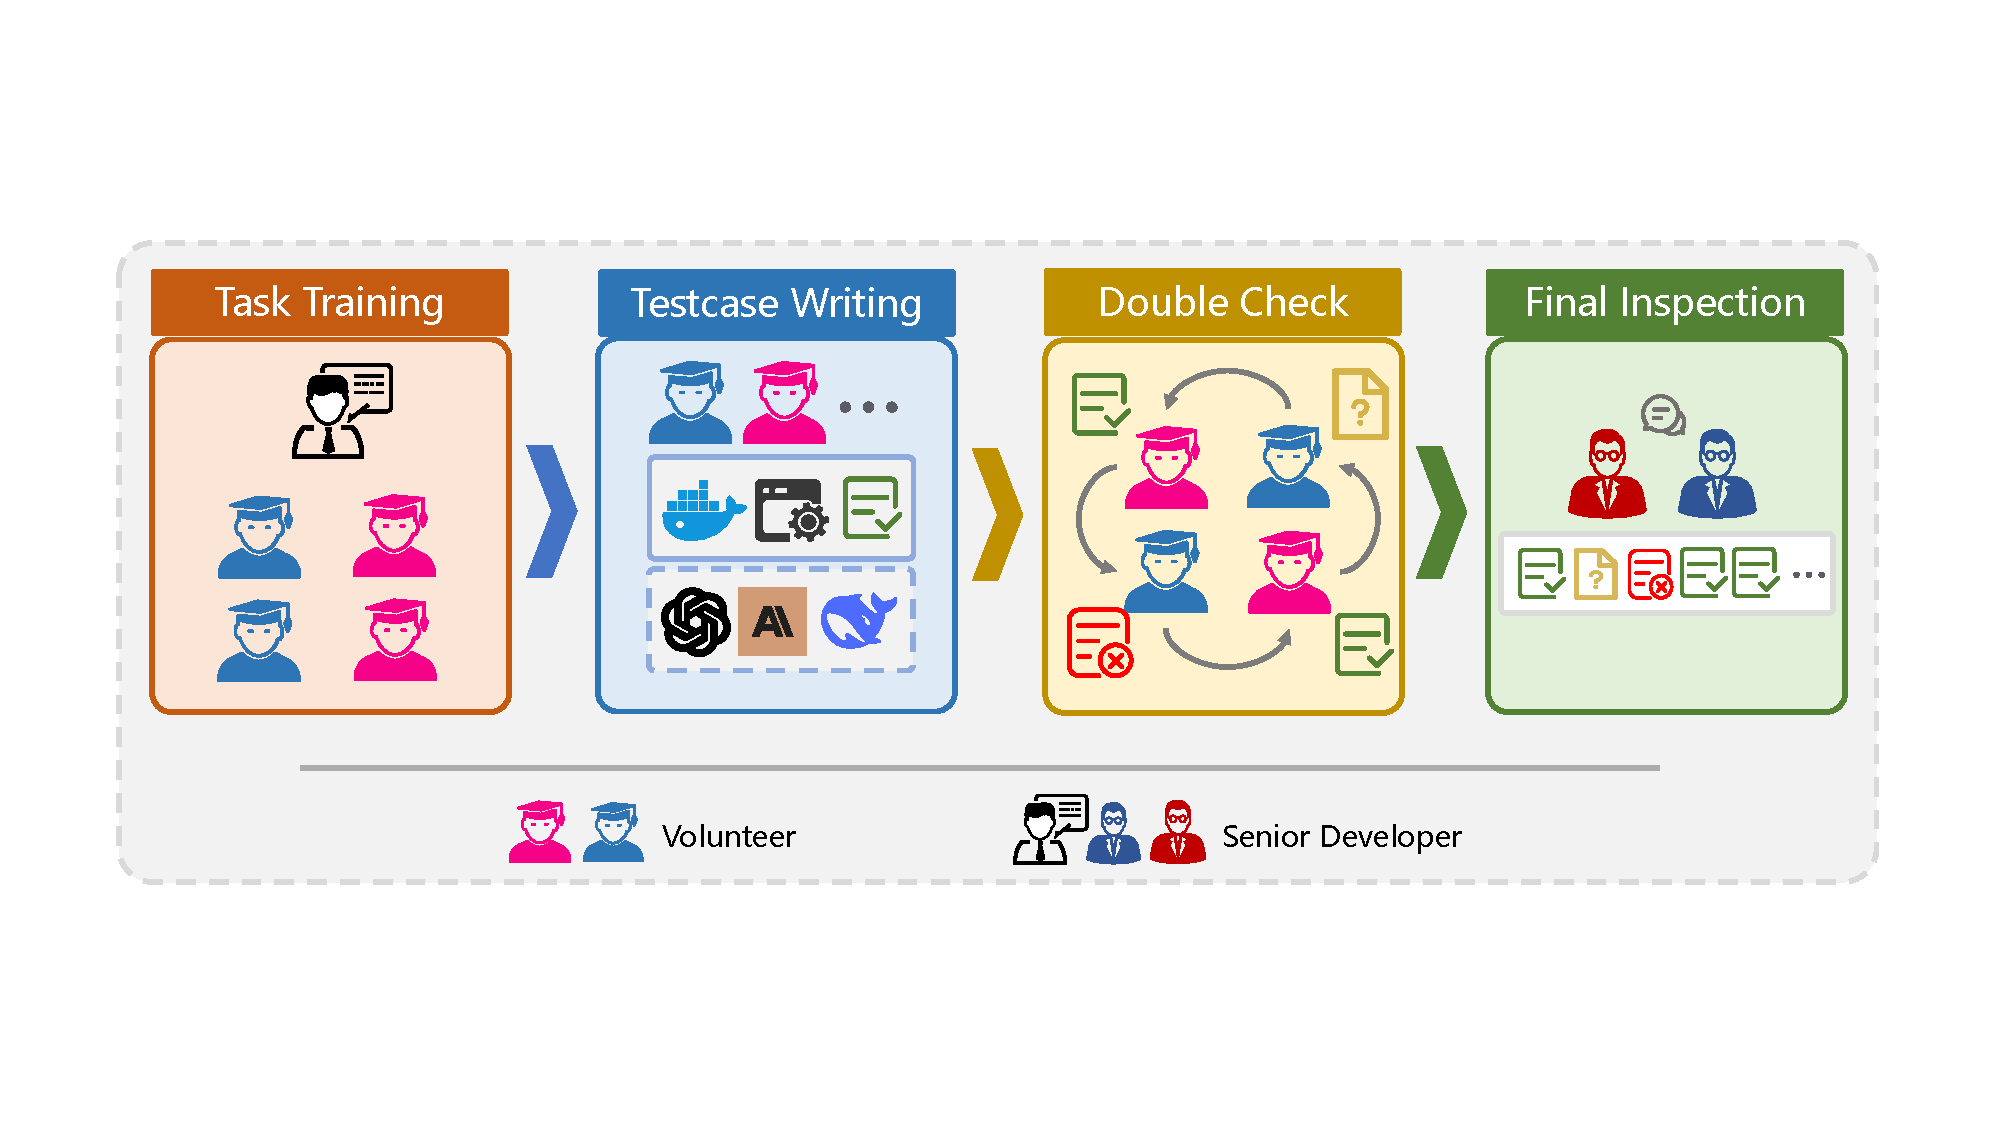
\includegraphics[width=0.8\linewidth]{figures/TestcaseGeneration.pdf}
    % \vspace{-1em}
    \caption{Workflow of Testcase Construction.}
   % \vspace{-0.5em}
    \label{fig:TestcaseGeneration}
\end{figure}


\section{Experimental Setup}

\subsection{Research Questions}
The research questions (RQs) explored in this study are as follows:
\begin{itemize}
    \item \textbf{RQ1:} How do the most advanced open-source and closed-source LLMs perform in repository-level code translation?
    \item \textbf{RQ2:} Can iteratively error-related information feedback to LLMs further improve its performance?
    \item \textbf{RQ3:} How does the complexity of the repository affect the performance of translation?
    \item \textbf{RQ4:} What are the main types of errors that occur in repository-level code translation?
\end{itemize}

% \subsection{Research Questions}  
% The research questions (RQs) explored in this study are as follows:
% \begin{enumerate}
%     \item \textbf{RQ1:} 目前最先进的开源和闭源模型在仓库级别代码翻译上的表现如何？
%     \item \textbf{RQ2:} 迭代地将error-related信息反馈给模型能否进一步提升其performance？
%     \item \textbf{RQ3:} repository-level code translation出现的错误主要有哪些?
%     \item \textbf{RQ4:} 对于 repository-level code translation特有的一些错误，有什么潜在的专门的解决措施？
% \end{enumerate}


\subsection{Model Selection}

For Python-to-Java repository-level code translation, the input length supported by traditional BERT-based pre-trained models is far from sufficient to meet the translation requirements. Due to the limitations of input and output window length, it is difficult to handle the long context of a repository. Therefore, in our experiments, we choose to evaluate the most advanced models currently available. The specific models are shown in Table~\ref{table:models}. We select four representative state-of-the-art open-source models and four popular closed-source models for evaluation.

% 对于python 到java的仓库级别代码翻译来说，传统的基于bert的预训练模型支持的输入长度远远不能够满足翻译的需求，受限于输入和输出的窗口长度限制，难以处理repo的长上下文。因此在我们的实验中，我们选择目前最先进的模型进行评估。具体模型如table:models中所示。我们挑选了四个具有代表性的最先进的开源模型,以及四个popular闭源模型用于评估

\begin{itemize}[left=10pt]
    \item \textbf{Llama-3.1-8B-Instruct}~\cite{Llama-3.1-8B-Instruct} is a Light-weight and ultra-fast version of Llama 3.1 family, which is a new state-of-the-art model from Meta. \textbf{Llama-3.1-70B-Instruct}~\cite{Llama-3.1-70B-Instruct} is a model with a larger number of parameters. \textbf{Llama-3.1-405B-Instruct}~\cite{Llama-3.1-405B-Instruct} is the first publicly released model that rivals top-tier closed-source AI models in areas such as common sense reasoning, controllability, mathematical capabilities, tool usage, and multilingual translation.
    \item \textbf{DeepSeek-V2.5}~\cite{deepseekv2} is a newly updated model from early September 2024. It is a combination of two models: DeepSeek-V2-Chat and DeepSeek-Coder-V2. This new model not only retains the general conversational capabilities of the original Chat model and the strong code handling abilities of the Coder model but also better aligns with human preferences. Additionally, its instruction-following capabilities have been significantly enhanced. DeepSeek-V2.5 is a strong Mixture-of-Experts (MoE) language model with only 21B activated parameters.
    \item \textbf{GPT-3.5-turbo}~\cite{gpt-3-5-turbo} is an accelerated version of the GPT-3.5 series developed by OpenAI. It improves reasoning speed and response efficiency while maintaining generation quality.
    \item \textbf{GPT-4-0125-Preview}~\cite{gpt-4-0125-preview} reduces instances of the model "lazily" failing to complete tasks and enhances its ability to execute tasks fully and accurately.
    \item \textbf{GPT-4o}~\cite{gpt-4o} successfully integrates text, vision, and audio, meaning it can accept any combination of text, audio, and images as input and generate any combination of text, audio, and images as output.
    \item \textbf{Claude-3.5-Sonnet}~\cite{Claude} is the first release in the Claude 3.5 model family. It sets new industry benchmarks for graduate-level reasoning (GPQA), undergraduate-level knowledge (MMLU), and coding proficiency (HumanEval).
\end{itemize}


% 翻译阶段
% 开源模型：codellama、DeepSeekcoder。。。，由于token长度限制，我们采用file-level的方式一个文件一个文件进行生成，同时为了能够让其参考到之前的信息，我们采用多轮对话的形式进行翻译
% 闭源模型：GPT-4o，Claude，DeepSeek-v2，GPT-3.5-turbo,前三者我们测了file和project level，gpt-3.5测了file-level
% 不同模型支持的token长度、资金消耗表


\begin{table}[t]
  \centering
  \footnotesize
  \setlength\tabcolsep{0.55pt}
  \caption{Overview of subject LLMs.\hy{July 2024, no '''} }
% \vspace*{-10pt}
\resizebox{0.7\columnwidth}{!}{
    \begin{tabular}{|l|c|c|c|c|c|}
    \hline
    \multicolumn{1}{|c|}{\textbf{Type}} & \multicolumn{1}{c|}{\textbf{Model}} & \multicolumn{1}{c|}{\textbf{Company}} & \multicolumn{1}{c|}{\textbf{Size}} & \multicolumn{1}{c|}{\textbf{Context Window}} & \multicolumn{1}{c|}{\textbf{Release Date}} \\
    \hline
    \hline
    \multirow{4}[2]{*}{\centering \makecell{Open\\Source}} & Llama-3.1-8B-Instruct~\cite{Llama-3.1-8B-Instruct} & \multirow{3}{*}{Meta} & 8B & 128K & July'2024 \\
    \cline{2-2}\cline{4-6}
     & Llama-3.1-70B-Instruct~\cite{Llama-3.1-70B-Instruct} &  & 70B & 128K & July'2024 \\
    \cline{2-2}\cline{4-6}
     & Llama-3.1-405B-Instruct~\cite{Llama-3.1-405B-Instruct} &  & 405B & 128K & July'2024 \\
    \cline{2-6}
     & DeepSeek-V2.5~\cite{deepseekv2} & DeepSeek & 236B* & 128K & Sep'2024 \\
    \hline
    \hline
    \multirow{4}[2]{*}{\centering \makecell{Closed\\Source}} & GPT-3.5-Turbo~\cite{gpt-3-5-turbo} & \multirow{3}{*}{OpenAI} & - & 16K & Sep'2021 \\
    \cline{2-2}\cline{4-6}
     & GPT-4-0125-Preview~\cite{gpt-4-0125-preview} &  & - & 128K & Dec'2023 \\
    \cline{2-2}\cline{4-6}
     & GPT-4o~\cite{gpt-4o} &  & - & 128K & May'2024 \\
    \cline{2-6}
     & Claude-3.5-Sonnet~\cite{claude-3-5-sonnet} & Anthropic & - & 200K & Jun'2024 \\
    \hline
    \end{tabular}}%
 \label{table:models}
% \vspace*{-2em}
\end{table}%

\subsection{Execution Environment}  
To prevent LLMs from generating malicious code that could execute on the local machine and cause damage, we run the translated code in an isolated environment. We use Docker~\cite{docker} as our code execution space. During the candidate repository filter stage, we need to check the passability of the Python projects. To this end, we install both Python 2.7.0 and 3.10 versions in the Docker environment, which can meet all requirements. For the passability tests of Java repositories, we consistently use JDK-11.0.23. Additionally, we bridge Docker's network with the local machine, allowing it to access the internet and ensuring that the dependencies in the pom.xml file can be successfully installed.
% 为了防止LLMs生成恶意代码在local机器上执行对local机器造成损害，我们运行翻译得到的代码都是在隔离环境中进行的，我们使用docker作为我们的代码执行空间。在Candidate repository filter阶段，我们需要对python repository进行testcase通过性测试，为此我们在docker环境中安装了2.7和3.10两个版本的python，能够满足所有需求。对于java repository的通过性测试，我们统一采用JDK-11.0.23。此外，我们将docker的网络和local机器进行桥接，使得其能够正常访问网络，保证pom.xml中的依赖能够被成功安装

\subsection{Evaluation Process}

As shown in Figure \ref{fig:EvaluationProcess}, we evaluate the performance of LLMs in repository-level code translation from two aspects: translation and debugging.

\textbf{Translation:} Given a Python repository, we place the corresponding Java test files in the system prompt of the LLMs as the translation target. Then, we input the code of the Python repository and the Java repository tree to the LLMs, requiring them to translate it into a series of Java code files. It is important to note that we only expect the LLMs to provide files under the \texttt{src/main/java} path or the \texttt{pom.xml} file. However, due to the limited instruction-following ability of some LLMs, they may generate extra files. Therefore, we need to perform a filtering process, retaining only the required files. Subsequently, we fill these translated code files into the unfinished Java repository, use the \texttt{docker cp} command to transfer them to the Docker container, and inside the Docker container, navigate to the project directory using \texttt{cd} and run \texttt{mvn clean test}~\cite{pan2024lost} to obtain the execution results. We then transfer the corresponding log files back to the local machine for information extraction.

\textbf{Debugging:} After obtaining the log files with the execution results of the LLM-translated code, we use regular expressions to extract the error-related information and feed it back to the LLMs. The LLMs analyze the cause of the errors based on the feedback and provide suggestions for modifications. We then replace the files in the previous Java repository with the updated ones. This process is repeated in a loop until the issues are resolved or the preset number of iterations is reached.

In our experiments, a complete round includes one translation and five iterations of debugging, which are labeled as \texttt{Iter 1-5}. To eliminate experimental randomness, we conduct three rounds of experiments under the same experimental setup, which is labeled as \texttt{Round 1-3} respectively. 

% 如图fig:EvaluationProcess所示，我们从翻译和debug两个方面来评估LLMs在仓库级别代码翻译上的表现。
% 翻译：给定一个python repository，我们将对应的java test files放在LLMs的system Prompt中作为LLMs的翻译目标，然后我们将python repository的代码和java repository tree作为LLMs的输入，要求LLMs对其进行翻译，得到一系列java代码文件，值得注意的是，我们只希望LLMs提供src/main/java路径下的文件或者是pom.xml文件，但受限于LLMs的指令跟随能力，一些LLMs可能会生成一些额外的文件，因此我们需要进行一次过滤，只保留我们要求的文件。随后我们将这些翻译得到的代码文件fill in unfinished java repository中，使用docker cp命令将其传输到docker容器中，在docker容器中cd到项目目录下，运行mvn clean test~\cite{pan2024lost}获取执行结果，然后将对应的log文件传输回local机器，进行信息提取。
% debug：在得到LLMs翻译之后的执行结果的log文件之后，我们使用正则表达式对其中的Error-related信息进行提取，将其反馈给模型，模型根据反馈的Error-related信息分析错误原因并给出修改意见，我们随后将其更新后的文件替换掉上一轮的java repository中的文件，然后往复这个循环，直至问题解决或达到预设的迭代轮次。

\begin{figure}
    \centering
    % \vspace{-10pt}
    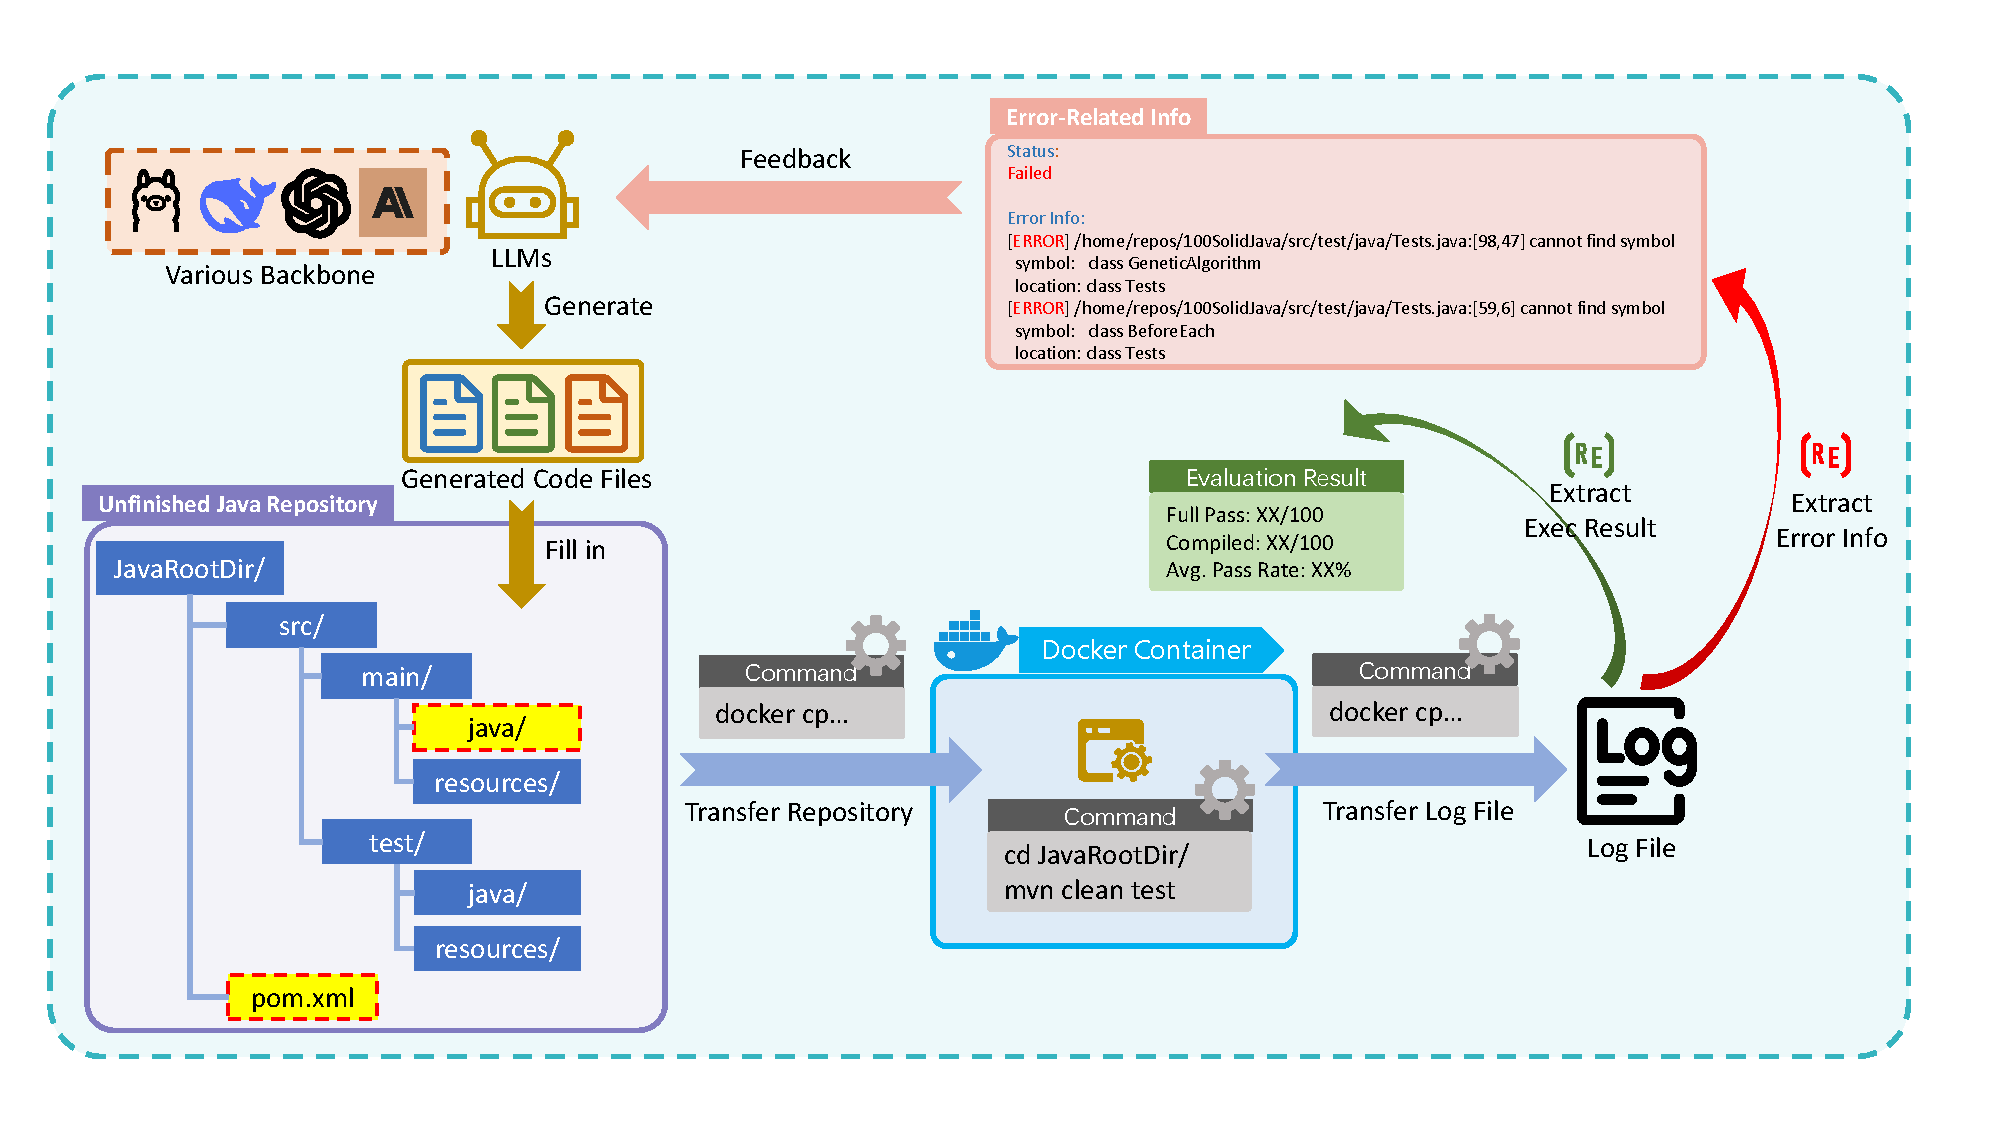
\includegraphics[width=\linewidth]{figures/EvaluationProcess.pdf}
    % \vspace{-1em}
    \caption{Overview of Evaluation Process.}
   % \vspace{-0.5em}
    \label{fig:EvaluationProcess}
\end{figure}

\subsection{Evaluation Metrics}
To better evaluate the performance of LLMs, we use the following metrics:
\begin{itemize}[left=10pt]
    \item \textbf{Full Pass:} This means the Java repository passes all test cases.
    \item \textbf{Compiled:} This means the Java repository is compilable, although it may not pass all test cases.
    \item \textbf{Avg.PR:} The full name is the average pass rate. Suppose the pass rate of one repository's test cases is denoted as \( PR_i \), then Avg.PR is calculated as \( \sum(PR_i) / \text{SampleNum} \), where SampleNum represents the number of repositories. In our benchmark, SampleNum is 100.
    \item \textbf{pass@3 for Full Pass:} The union of the repositories that achieve a full pass across the three rounds of experiments.
    \item \textbf{pass@3 for Compiled:} The union of the repositories that are compiled successfully across the three rounds of experiments.
\end{itemize}

% 在我们的实验中，一轮完整的实验包括一次翻译和5次迭代的debug。为了消除实验的偶然性，我们在相同实验设置下进行了三轮实验。结束以上实验之后我们会统计相应的实验结果，我们的指标有以下几个：
% Full Pass: 这意味着java repository通过了全部的测试用例
% Compiled：这意味这java repository是可编译的，尽管可能没有通过全部的测试用例
% Pass Rate：当前repository通过的测试用例个数/总个数
% Avg. Pass Rate: 全部的sample（100个）的平均pass rate， 也就是sum(PassRate_i)/SampleNum
% pass@3 of full pass: 三轮实验full pass的repository的并集
% pass@3 of compiled： 三轮实验编译通过的repository的并集


\section{Evaluation Results}
\subsection{Performance of Translation}  

Table \ref{table:TranslationResults} highlights the performance disparities among different large language models (LLMs) across three rounds of code translation. Claude-3.5-Sonnet consistently demonstrates superior performance, with 9 out of 100 repositories achieving a full pass in Round 1, 7 in Round 2, and 6 in Round 3. This model also maintains the highest average pass rate of 16.5\%, indicating strong code generation and instruction-following capabilities, particularly in complex repository-level translation tasks.

In contrast, models like Llama-3.1-8B-Inst show significantly poorer results, with zero full passes and a 0.0\% average pass rate. This may indicate limitations in both code generation and instruction-following abilities. The smaller parameter size (8B) could be a contributing factor, as it might lack the capacity to generate syntactically correct and semantically meaningful code at scale. Additionally, Llama-3.1-8B-Inst may struggle with understanding and following complex instructions required for tasks like code translation, where precision and context retention are critical. This is further evidenced by its inability to successfully compile any of the repositories.

The larger models like Llama-3.1-405B-Inst perform slightly better but still fall short, suggesting that even with more parameters, the instruction-following capabilities are not as strong as those of models like Claude-3.5-Sonnet. This highlights that both model size and fine-tuning for code-specific tasks play key roles in achieving higher pass rates and overall better performance in code translation tasks.

\begin{center}
    \begin{myboxc} \textbf{RQ1 Summary: } %cd
    Both open-source and closed-source LLMs, regardless of their parameter size, perform poorly on RepoTranBench. The strongest closed-source model, Claude-3.5-Sonnet, can fully pass only 7 out of 100 repositories on average. Similarly, the best open-source LLMs, DeepSeek-V2.5 and Llama-3.1-405B-Inst, can fully pass only 3 repositories on average.
    \end{myboxc} %cd
\end{center}


\begin{table}[t]
  \centering
  \footnotesize
  \setlength\tabcolsep{1.5pt}
  \caption{Performance comparison across different LLMs in three rounds of translation.}
% \vspace*{-10pt}
\resizebox{\columnwidth}{!}{
    \begin{tabular}{l|c|c|c|c|c|c|c|c|c|c|c|c|c|c}
    \hline
    \textbf{Model} & \multicolumn{3}{c|}{\textbf{Round 1}} & \multicolumn{3}{c|}{\textbf{Round 2}} & \multicolumn{3}{c|}{\textbf{Round 3}} & \multicolumn{2}{c|}{\textbf{pass@3}} & \multicolumn{3}{c}{\textbf{Average}} \\
    \cline{2-15}
    & \textbf{Full Pass} & \textbf{Compiled} & \textbf{Avg.PR} & \textbf{Full Pass} & \textbf{Compiled} & \textbf{Avg.PR} & \textbf{Full Pass} & \textbf{Compiled} & \textbf{Avg.PR} & \textbf{Full Pass} & \textbf{Compiled} & \textbf{Full Pass} & \textbf{Compiled} & \textbf{Avg.PR} \\
    \hline
    Llama-3.1-8B-Inst & 0/100 & 0/100 & 0.0\% & 0/100 & 0/100 & 0.0\% & 0/100 & 0/100 & 0.0\% & 0/100 & 0/100 & 0/100 & 0/100 & 0.0\% \\
    Llama-3.1-70B-Inst & 2/100 & 2/100 & 1.0\% & 0/100 & 3/100 & 0.7\% & 2/100 & 3/100 & 2.1\% & 3/100 & 6/100 & 1/100 & 3/100 & 1.3\% \\
    Llama-3.1-405B-Inst & 2/100 & 5/100 & 3.8\% & 2/100 & 7/100 & 5.4\% & 4/100 & 5/100 & 4.9\% & 4/100 & 10/100 & 3/100 & 6/100 & 4.7\% \\
    DeepSeek-V2.5 & 5/100 & 14/100 & 9.4\% & 2/100 & 8/100 & 2.9\% & 2/100 & 14/100 & 6.3\% & 6/100 & 20/100 & 3/100 & 12/100 & 6.2\% \\
    \hline
    GPT-3.5-Turbo & 0/100 & 2/100 & 0.0\% & 1/100 & 3/100 & 2.3\% & 1/100 & 2/100 & 1.0\% & 1/100 & 5/100 & 1/100 & 2/100 & 1.1\% \\
    GPT-4-0125-Preview & 2/100 & 3/100 & 1.0\% & 3/100 & 5/100 & 3.1\% & 2/100 & 5/100 & 1.7\% & 4/100 & 9/100 & 2/100 & 4/100 & 2.0\% \\
    GPT-4o & 5/100 & 8/100 & 5.7\% & 3/100 & 9/100 & 6.5\% & 4/100 & 10/100 & 7.1\% & 8/100 & 19/100 & 4/100 & 9/100 & 6.4\% \\
    Claude-3.5-Sonnet & 9/100 & 32/100 & 19.6\% & 7/100 & 24/100 & 13.8\% & 6/100 & 29/100 & 16.1\% & 12/100 & 42/100 & 7/100 & 28/100 & 16.5\% \\
    \hline
    \end{tabular}}%
 \label{table:TranslationResults}
% \vspace*{-2em}
\end{table}



\subsection{Performance of Iterative Debugging}  

As shown in Table.\ref{table:IterDebugResults}, by providing error-related feedback, most models show improvements in full pass rates through iterative debugging. However, models with weaker instruction-following capabilities, such as Llama-3.1-8B-Inst, consistently fail to improve, resulting in an average full pass rate of 0 across all rounds and iterations. Even after five iterative debugging steps, Llama-3.1-8B-Inst shows no meaningful progress in any of the rounds or Pass@3 scores. In contrast, larger models like Llama-3.1-405B-Inst and instruction-tuned models like GPT-4o exhibit significant improvements. For instance, GPT-4o's full pass rate increases from 7 to 20 by the third round, and its Pass@3 rate jumps from 8 to 33 after five iterations, demonstrating the model's enhanced ability to learn from iterative feedback.

Models like Claude-3.5-Sonnet also show notable progress, particularly in earlier rounds, where it manages to improve from a raw pass rate of 9 to 16 in Round 1 and 12 to 22 in Pass@3 after five iterations. Similarly, GPT-4-0125-Preview sees steady improvement, although it lags slightly behind GPT-4o in terms of overall gains. DeepSeek-V2.5 also shows moderate improvements, especially in Pass@3, increasing from 6 to 11 across iterations, but its performance is less consistent compared to GPT-series models.

However, despite these gains, the overall performance of most LLMs remains below optimal levels. Even with iterative debugging, many models struggle with complex debugging tasks, as reflected in relatively low final pass rates. This highlights the continuing need for advancements in error comprehension and instruction-following capabilities to reliably handle more challenging debugging scenarios across all iterations.


\begin{center}
    \begin{myboxc} \textbf{RQ2 Summary: } %cd
    By providing error-related feedback, most models show improvements in full pass rates through iterative debugging. However, models with weaker instruction-following capabilities still fail to improve. Although iterative debugging leads to improvements, the overall performance of current LLMs remains low.
    \end{myboxc} %cd
\end{center}

\begin{table}[t]
  \centering
  \footnotesize
  \setlength\tabcolsep{1.5pt}
  \caption{Performance comparison across different LLMs in three rounds and 5 iterative debugging.}
\resizebox{\columnwidth}{!}{
    \begin{tabular}{l|cccccc|cccccc|cccccc|cccccc|cccccc}
    \hline
    \textbf{Model} & \multicolumn{6}{c|}{\textbf{Round 1}} & \multicolumn{6}{c|}{\textbf{Round 2}} & \multicolumn{6}{c|}{\textbf{Round 3}} & \multicolumn{6}{c|}{\textbf{Pass@3}} & \multicolumn{6}{c}{\textbf{Average}} \\
    \cline{2-31}
    & \textbf{Raw} & \textbf{Iter 1} & \textbf{Iter 2} & \textbf{Iter 3} & \textbf{Iter 4} & \textbf{Iter 5} & \textbf{Raw} & \textbf{Iter 1} & \textbf{Iter 2} & \textbf{Iter 3} & \textbf{Iter 4} & \textbf{Iter 5} & \textbf{Raw} & \textbf{Iter 1} & \textbf{Iter 2} & \textbf{Iter 3} & \textbf{Iter 4} & \textbf{Iter 5} & \textbf{Raw} & \textbf{Iter 1} & \textbf{Iter 2} & \textbf{Iter 3} & \textbf{Iter 4} & \textbf{Iter 5} & \textbf{Raw} & \textbf{Iter 1} & \textbf{Iter 2} & \textbf{Iter 3} & \textbf{Iter 4} & \textbf{Iter 5} \\
    \hline
    Llama-3.1-8B-Inst & 0/100 & 0/100 & 0/100 & 0/100 & 0/100 & 0/100 & 0/100 & 0/100 & 0/100 & 0/100 & 0/100 & 0/100 & 0/100 & 0/100 & 0/100 & 0/100 & 0/100 & 0/100 & 0/100 & 1/100 & 1/100 & 1/100 & 1/100 & 0/100 & 0/100 & 0/100 & 0/100 & 0/100 & 0/100 & 0/100 \\
    Llama-3.1-70B-Inst & 2/100 & 4/100 & 5/100 & 6/100 & 6/100 & 8/100 & 0/100 & 1/100 & 1/100 & 1/100 & 1/100 & 1/100 & 2/100 & 1/100 & 1/100 & 1/100 & 4/100 & 6/100 & 3/100 & 5/100 & 6/100 & 6/100 & 9/100 & 13/100 & 1/100 & 2/100 & 2/100 & 3/100 & 4/100 & 5/100 \\
    Llama-3.1-405B-Inst & 2/100 & 1/100 & 1/100 & 6/100 & 7/100 & 9/100 & 2/100 & 3/100 & 4/100 & 7/100 & 9/100 & 12/100 & 4/100 & 4/100 & 6/100 & 7/100 & 8/100 & 8/100 & 4/100 & 6/100 & 9/100 & 15/100 & 18/100 & 21/100 & 3/100 & 3/100 & 4/100 & 7/100 & 8/100 & 10/100 \\
    DeepSeek-V2.5 & 5/100 & 6/100 & 7/100 & 9/100 & 11/100 & 13/100 & 2/100 & 3/100 & 7/100 & 9/100 & 11/100 & 11/100 & 2/100 & 1/100 & 3/100 & 7/100 & 7/100 & 9/100 & 6/100 & 7/100 & 12/100 & 18/100 & 20/100 & 22/100 & 3/100 & 3/100 & 6/100 & 8/100 & 10/100 & 11/100 \\
    \hline
    GPT-3.5-Turbo & 0/100 & 1/100 & 2/100 & 3/100 & 4/100 & 7/100 & 1/100 & 1/100 & 3/100 & 3/100 & 5/100 & 6/100 & 1/100 & 2/100 & 2/100 & 3/100 & 4/100 & 5/100 & 1/100 & 3/100 & 5/100 & 7/100 & 10/100 & 14/100 & 1/100 & 1/100 & 2/100 & 3/100 & 4/100 & 6/100 \\
    GPT-4-0125-Preview & 2/100 & 3/100 & 3/100 & 3/100 & 5/100 & 6/100 & 3/100 & 3/100 & 5/100 & 6/100 & 7/100 & 7/100 & 2/100 & 5/100 & 9/100 & 9/100 & 12/100 & 14/100 & 4/100 & 9/100 & 13/100 & 14/100 & 19/100 & 20/100 & 2/100 & 4/100 & 6/100 & 6/100 & 8/100 & 9/100 \\
    GPT-4o & 5/100 & 5/100 & 12/100 & 17/100 & 21/100 & 22/100 & 3/100 & 6/100 & 10/100 & 13/100 & 16/100 & 18/100 & 4/100 & 5/100 & 11/100 & 13/100 & 16/100 & 20/100 & 8/100 & 13/100 & 23/100 & 29/100 & 33/100 & 33/100 & 4/100 & 5/100 & 11/100 & 14/100 & 18/100 & 20/100 \\
    Claude-3.5-Sonnet & 9/100 & 11/100 & 14/100 & 14/100 & 15/100 & 16/100 & 7/100 & 8/100 & 10/100 & 10/100 & 11/100 & 12/100 & 6/100 & 8/100 & 13/100 & 16/100 & 17/100 & 17/100 & 12/100 & 14/100 & 19/100 & 20/100 & 21/100 & 22/100 & 7/100 & 9/100 & 12/100 & 13/100 & 14/100 & 15/100 \\
    \hline
    \end{tabular}}%
 \label{table:IterDebugResults}
\end{table}


% \begin{figure}
%     \centering
%     % \vspace{-10pt}
%     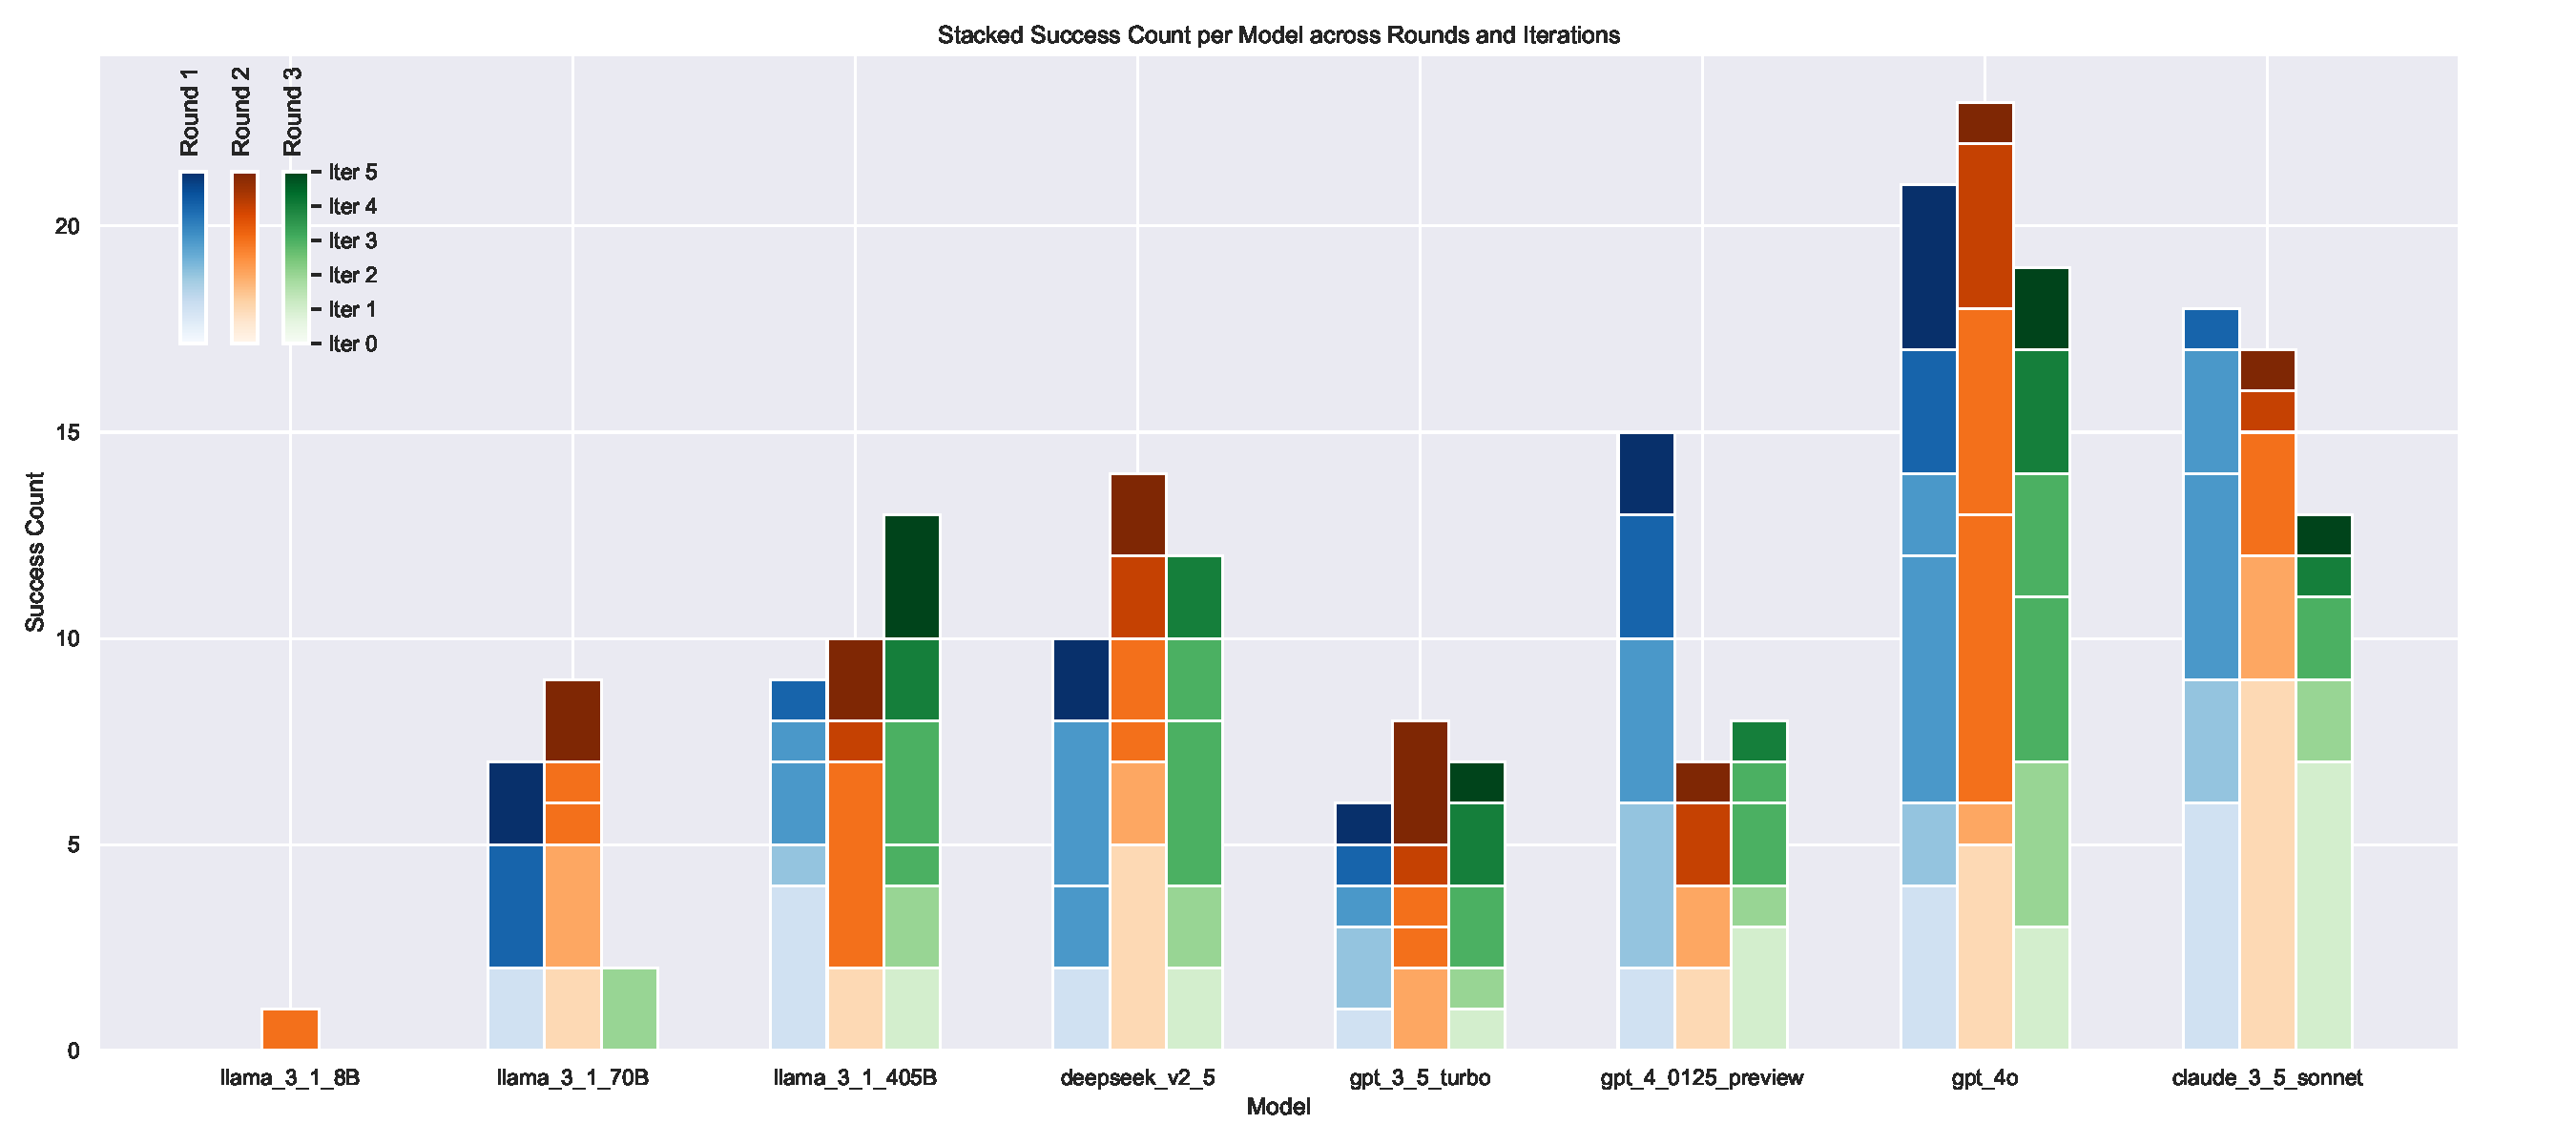
\includegraphics[width=\linewidth]{figures/ModelIter.pdf}
%     % \vspace{-1em}
%     \caption{Success Count per Model across Rounds and Iterations.}
%    % \vspace{-0.5em}
%     \label{fig:ModelIter}
% \end{figure}


\subsection{Effect of the Complexity}  
As shown in Figure.~\ref{fig:AffectOfComplexity}, the complexity of a repository significantly impacts the success of its translation. More complex repositories, indicated by higher counts of tokens, lines, functions, classes, and imports, tend to result in lower success rates during translation. Specifically, as the number of tokens and structural components increases, the translation process becomes more challenging, leading to a noticeable rise in failure cases. This suggests that complexity introduces additional obstacles in accurately capturing the functionality and structure of the original repository, making it more prone to errors and inconsistencies during translation.

\begin{center}
    \begin{myboxc} \textbf{RQ3 Summary: } %cd
    Higher repository complexity leads to lower translation success rates, with more tokens, lines, functions, classes, and imports increasing the likelihood of failures.
    \end{myboxc} %cd
\end{center}

\begin{figure}
    \centering
    % \vspace{-10pt}
    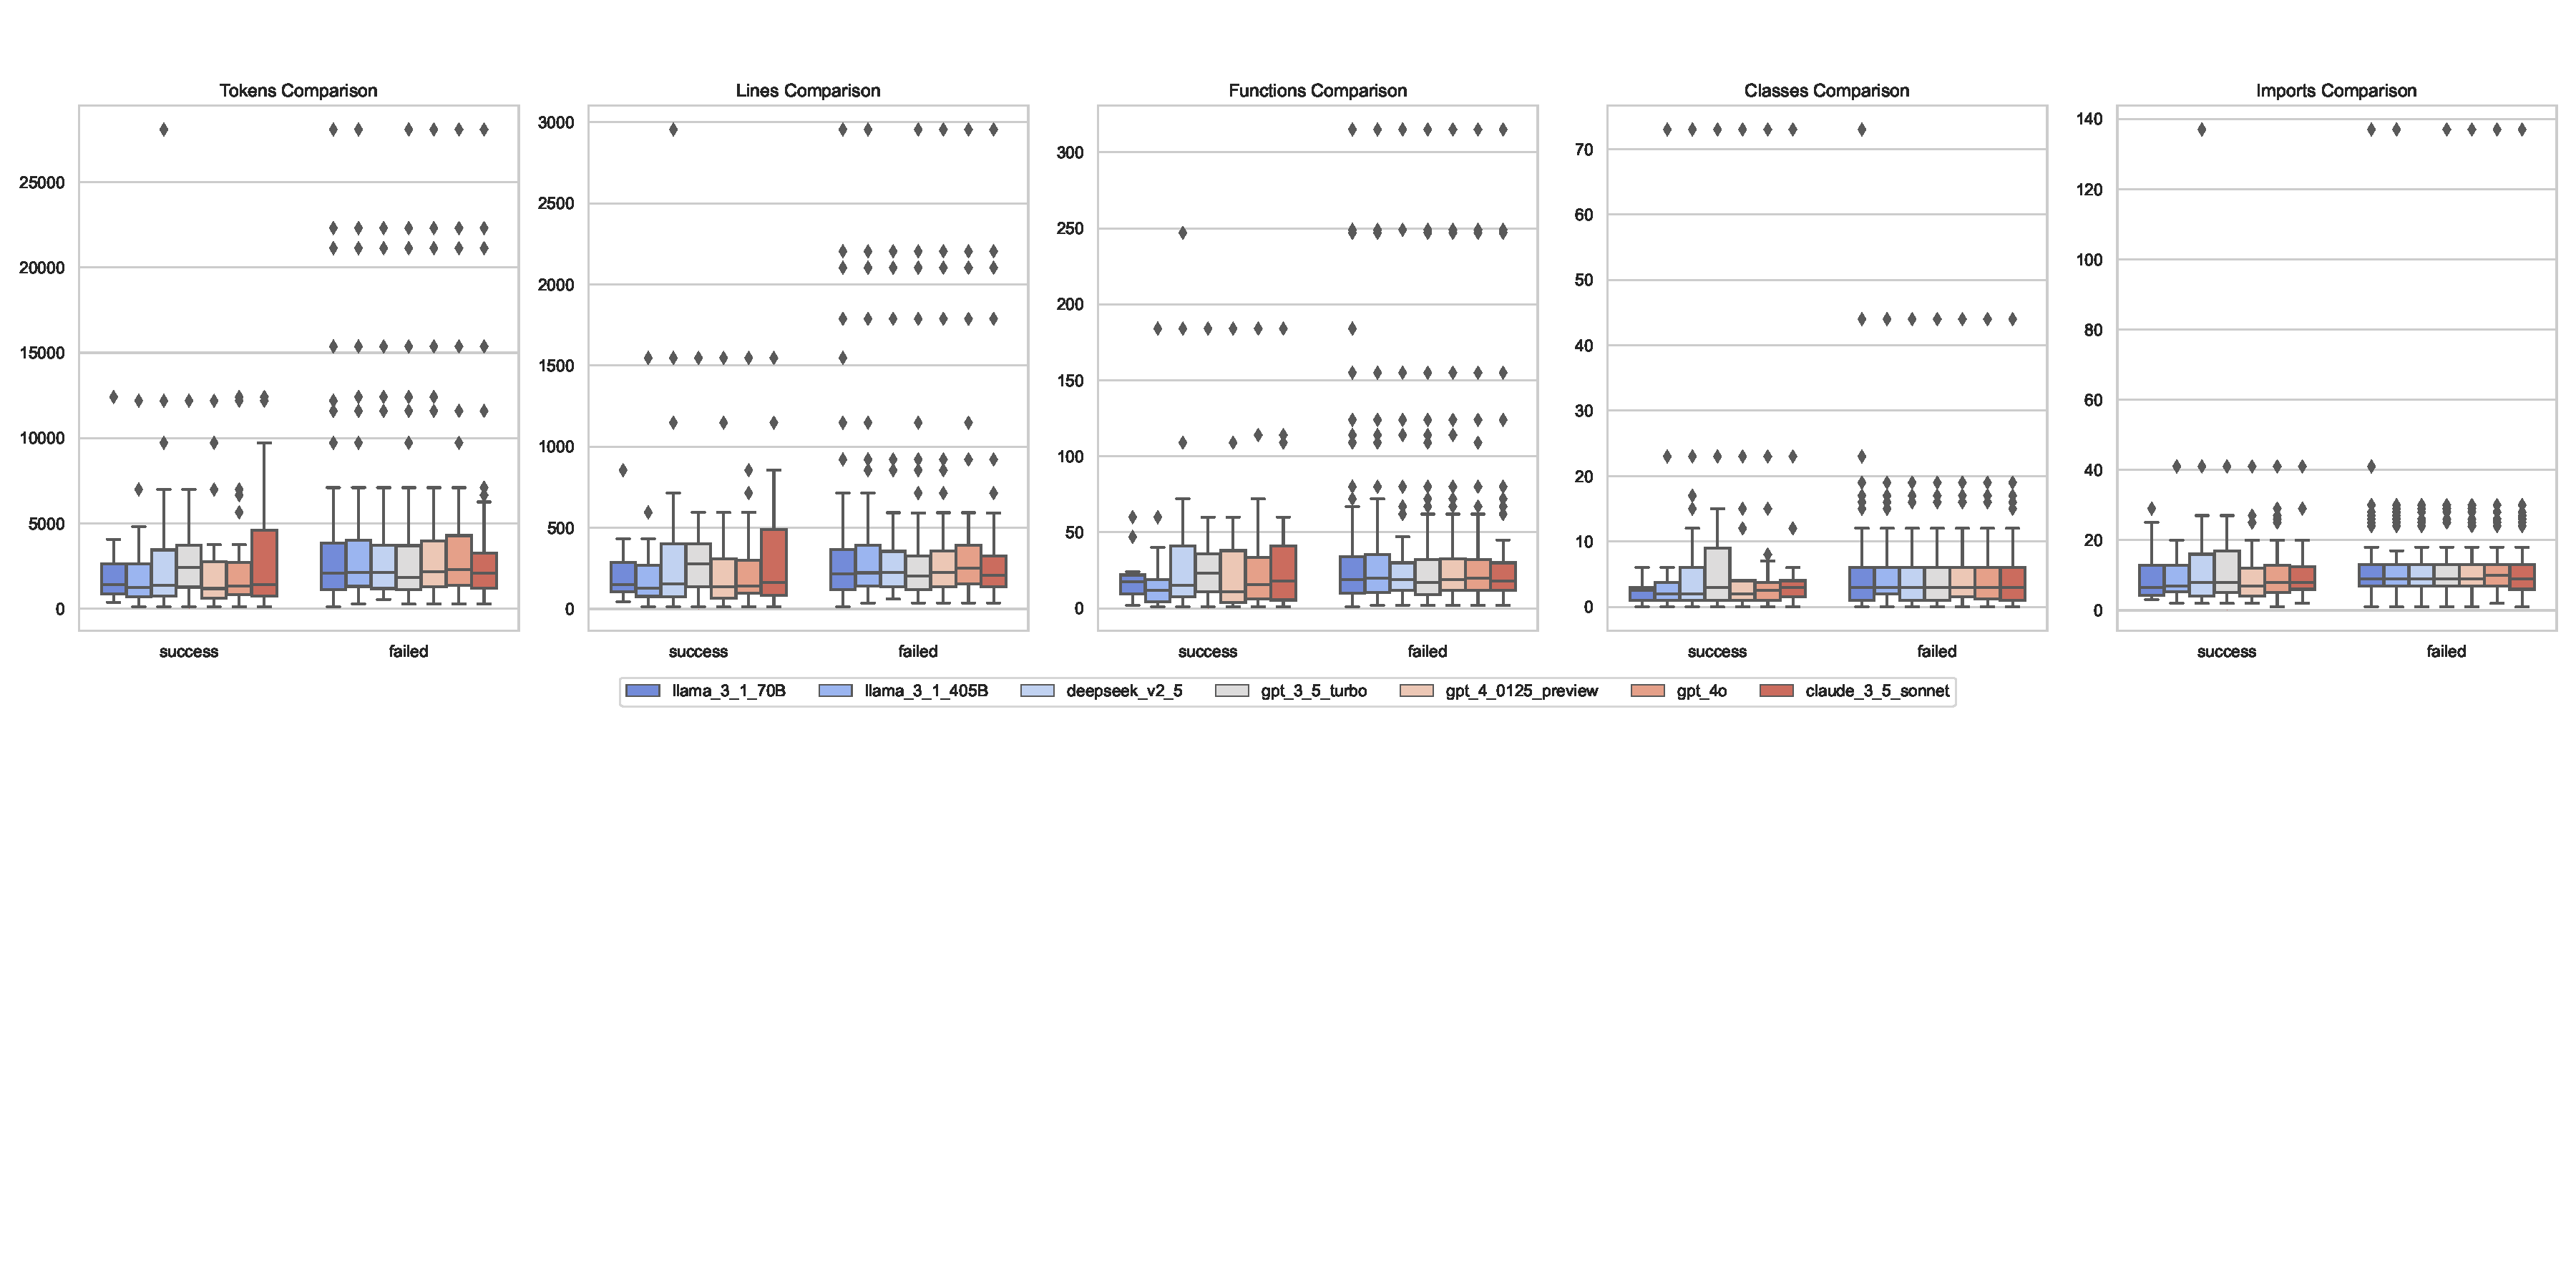
\includegraphics[width=\linewidth]{figures/AffectOfComplexity.pdf}
    % \vspace{-1em}
    \caption{Affect of the Complexity.}
   % \vspace{-0.5em}
    \label{fig:AffectOfComplexity}
\end{figure}


\subsection{Error Analysis}
We enlist volunteers to conduct a thorough error analysis over three rounds of experiments, ultimately identifying the following common errors in repository-level code translation, which are classified into five categories.

\begin{figure}
    \centering
    % \vspace{-10pt}
    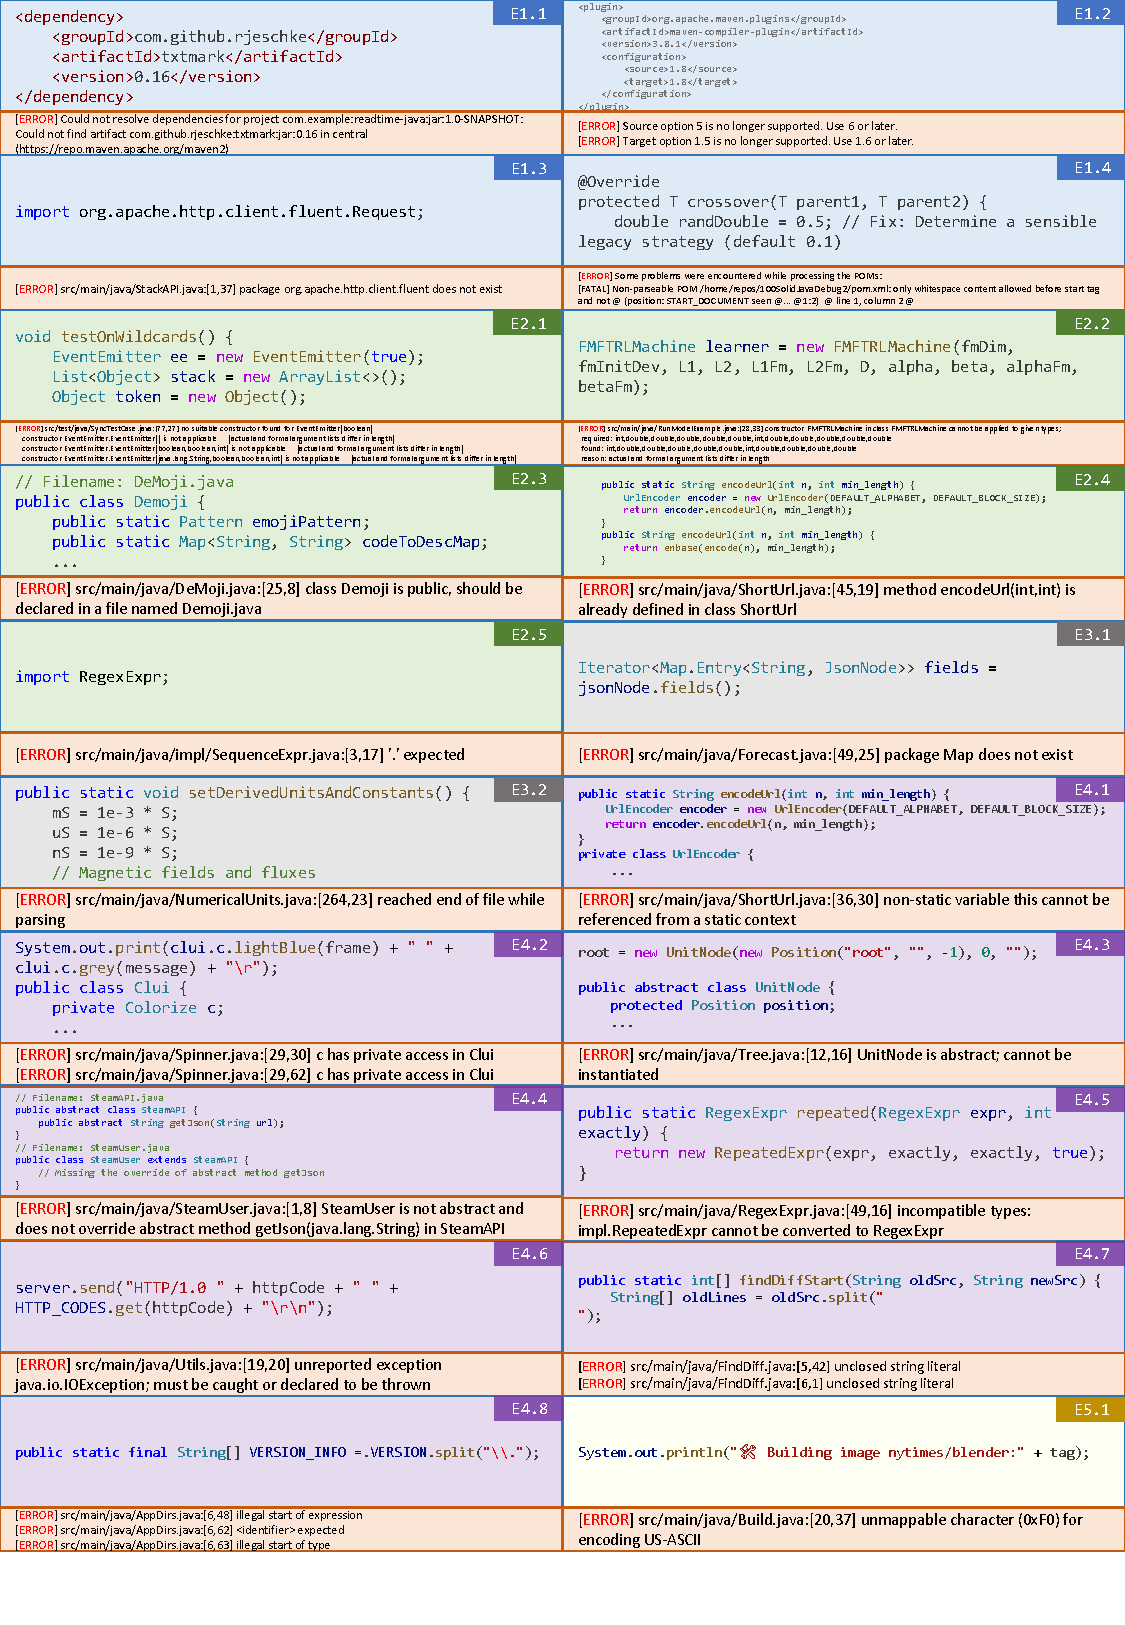
\includegraphics[width=\linewidth]{figures/ErrorCase1.pdf}
    % \vspace{-1em}
    \caption{Error Case.}
   % \vspace{-0.5em}
    \label{fig:ErrorCase}
\end{figure}

\textbf{E1. Configuration File (pom.xml) Issues:}
These errors arise from misconfigurations in the project’s \texttt{pom.xml} file, causing failures in dependency resolution, Java version mismatches, or other configuration-related issues.

\begin{itemize}[left=10pt]
    \item \textbf{E1.1. Unresolved Dependency Error:}  
    This error occurs because the artifact can not be found in the central Maven repository. As a result, Maven is unable to resolve the necessary dependencies for the project.
    
    \item \textbf{E1.2. Unsupported Java Version Error:}  
    Since the \texttt{pom.xml} file does not explicitly specify the Java version, Maven defaults to a version. Historically, Maven's default source and target version was 1.5, which might not match the required version. To resolve this issue, the Java version must be explicitly set in the \texttt{pom.xml} file, for example, specifying version 1.8 as shown in the figure.
    
    \item \textbf{E1.3. Missing or Misconfigured Dependency:}  
    The error message indicates that the package \texttt{org.apache.http.client.fluent} is not found in the project. This happens when the required dependency for Apache HttpClient Fluent API is missing or improperly configured in the build file (such as \texttt{pom.xml} when using Maven).
    
    \item \textbf{E1.4. Inappropriate Content in config file:}  
    The issue arises when content that does not belong in the \texttt{pom.xml} file is added, leading to errors during project setup.
\end{itemize}

\textbf{E2. Limited Understanding:}
These errors are caused by a lack of familiarity with class structures, constructor arguments, and Java syntax, leading to issues such as incorrect class instantiation or naming conventions.

\begin{itemize}[left=10pt]
    \item \textbf{E2.1. Calling a Non-existent Constructor:}  
    The error message shows that the EventEmitter constructor \texttt{EventEmitter ee = new EventEmitter(true);} does not match any available constructors in the EventEmitter class. Though the class has multiple constructors, none accepts a single boolean argument.
    
    \item \textbf{E2.2. Incorrect Constructor Arguments:}  
    The code attempts to instantiate an \texttt{FMFTRLMachine} object with a constructor whose argument list does not match the expected parameters. The \texttt{FMFTRLMachine} constructor requires 12 parameters of types \texttt{int, double, double, double, double, double, int, double, double, double, double, double}. However, only 11 arguments are provided, causing a mismatch in the constructor signature and leading to a compile-time error.
    
    \item \textbf{E2.3. Mismatch Between File Name and Class Name:}  
    The class \texttt{Demoji} is declared as \texttt{public}, but the file name is incorrectly spelled as \texttt{DeMoji.java}. In Java, the file name must exactly match the class name, including case sensitivity, for public classes. Hence, the file should be renamed to \texttt{Demoji.java} to prevent the compiler from throwing an error.
    
    \item \textbf{E2.4. Method Redefinition:}  
    The error occurs because the class \texttt{ShortUrl} contains two methods with the same name \texttt{encodeUrl(int, int)}, leading to a conflict in the method signature. Java allows method overloading if the parameter types or number of parameters differ. However, in this case, both methods have identical signatures, causing confusion for the compiler.
    
    \item \textbf{E2.5. Incorrect Import Statement:}  
    The error \texttt{"'.' expected"} in the context of \texttt{import RegexExpr;} indicates that Java expects a dot (\texttt{.}) to reference a package. Since \texttt{RegexExpr} is a class and does not need to be imported, the solution is to remove the import statement.
\end{itemize}

\textbf{E3. Incomplete Code Generation:}
These errors result from incomplete code generation due to limitations in word count or missing elements such as import statements, which lead to compilation issues.

\begin{itemize}[left=10pt]
    \item \textbf{E3.1. Missing Necessary Import Statement:}  
    The error message \texttt{"package Map does not exist"} arises because the Map interface is not recognized by the Java compiler. The Map interface belongs to the \texttt{java.util} package and the lack of an import statement for this package causes the error.
    
    \item \textbf{E3.2. Premature Termination of Code:}  
    In this code snippet, the generated code is prematurely terminated due to the limitation on the maximum length of word generation. As a result, the complete code is not generated.
\end{itemize}

\textbf{E4. Syntax Issues (“Next Code Token” Predictors):}
These errors are caused by inconsistent language features, which lead to referencing non-static classes from static contexts or failing to match return types, etc.

\begin{itemize}[left=10pt]
    \item \textbf{E4.1. Referencing Non-static Class from Static Context:}  
    The error \texttt{"non-static variable this cannot be referenced from a static context"} occurs because the code attempts to create an instance of an inner class (\texttt{UrlEncoder}) inside a static method (\texttt{encodeUrl}), but inner classes require an instance of the enclosing class to access their non-static members.
    
    \item \textbf{E4.2. Accessing Private Members:}  
    The error message indicates that the member variable \texttt{c} in the \texttt{Clui} class is private and cannot be accessed directly from another class (such as \texttt{Spinner.java}).
    
    \item \textbf{E4.3. Instantiating Abstract Class:}  
    The error occurs because the code attempts to instantiate an abstract class (\texttt{UnitNode}). In Java, abstract classes cannot be instantiated directly and must be extended by a subclass that provides implementations for the abstract methods.

    \item \textbf{E4.4. Missing Method Implementation:}  
    The error occurs because the subclass \texttt{SteamUser} does not provide an implementation for the abstract method \texttt{getJson(String url)} declared in the abstract class \texttt{SteamAPI}. In Java, if a class extends an abstract class, it must either provide concrete implementations for all abstract methods or be declared as abstract. Since \texttt{SteamUser} is not declared abstract, the compiler expects it to implement the \texttt{getJson} method from \texttt{SteamAPI}. To resolve the error, the subclass must override and implement the missing method.
    
    \item \textbf{E4.5. Incorrect Return Type:}  
    The method \texttt{repeated()} is expected to return an instance of \texttt{RegexExpr}, but it returns an instance of \texttt{RepeatedExpr}. This mismatch between the expected and actual return types leads to a type incompatibility.
    
    \item \textbf{E4.6. Missing Expected Exception:}  
    The method \texttt{server.send()} is expected to throw an \texttt{IOException}, but it does not throw the exception as anticipated.
    
    \item \textbf{E4.7. Incorrect Newline Representation:}  
    In Java, a newline character inside a string is represented by the escape sequence \texttt{\textbackslash n}. However, the generated code incorrectly represents this in the \texttt{split()} method, leading to errors.
    
    \item \textbf{E4.8. Invalid Syntax:}  
    A dot (\texttt{.}) is incorrectly placed after the equals sign (\texttt{=}), causing the Java compiler to throw a syntax error. The correct syntax should place the dot immediately after the object or class from which \texttt{VERSION} is being referenced.
\end{itemize}

\textbf{E5. Encoding Issues:}
These errors occur due to incompatible repository encoding formats, which can lead to issues when special characters, such as emojis, are used.

\begin{itemize}[left=10pt]
    \item \textbf{E5.1. Encoding Missing:}  
    The error \texttt{"unmappable character (0xF0) for encoding US-ASCII"} occurs because the file is being compiled using the US-ASCII encoding, which does not support certain characters, such as emojis. Since emojis are Unicode characters, US-ASCII cannot represent them. The solution is to add \texttt{<encoding>UTF-8</encoding>} in the \texttt{<configuration>} tag of the \texttt{pom.xml} file to resolve this issue.
\end{itemize}

\begin{center}
    \begin{myboxc} \textbf{RQ4 Summary: } %cd
    Repository-level code translation faces significant challenges due to inconsistent language features, complex dependency management, and incompatible library usage across projects. These factors increase the difficulty of accurately translating code at a larger scale, making it more prone to failure.
    \end{myboxc} %cd
\end{center}


% E1. 配置文件(pom.xml)问题：
% E1.1. Unresolved Dependency Error
% The error occurs because the artifact \texttt{com.github.rjeschke:txtmark:jar:0.16} could not be found in the central Maven repository at \texttt{https://repo.maven.apache.org/maven2}. This prevents Maven from resolving the dependencies required for the project \texttt{com.example:readtime-java:jar:1.0-SNAPSHOT}.

% E1.2. Unsupported Java Version Error
% there is no explicit configuration for the Java version in the pom.xml file, Maven uses a default. Historically, Maven’s default source and target version was 1.5,和实际的版本不相符。为了解决这一问题，我们需要补上相应的版本信息，比如图中所示的将版本显示地设置为1.8即可。

% E1.3. dependency missing或没有被正确配置
% The error message indicates that the package org.apache.http.client.fluent is not found in the project. This happens when the required dependency for Apache HttpClient Fluent API is missing or not properly configured in your project’s build file (pom.xml if you are using Maven).

% E1.4. 将不合适的内容写入pom.xml
% 将不属于pom.xml的内容写入pom.xml文件中


% E2. 理解能力有限
% E2.1 调用不存在的构造函数
% The error message indicates that the EventEmitter constructor used in the line EventEmitter ee = new EventEmitter(true); doesn't match any of the available constructors in the EventEmitter class. The EventEmitter class seems to have multiple constructors, but none that accepts a single boolean argument.

% E2.2 调用函数传参不正确
% This piece of code is attempting to instantiate an object of the class `FMFTRLMachine` using a constructor that does not match the expected argument list. The error indicates that the constructor of the `FMFTRLMachine` class requires 12 parameters of types `int, double, double, double, double, double, int, double, double, double, double, double`. However, the provided instantiation is missing one argument, as it supplies only 11 parameters of types `int, double, double, double, double, double, int, double, double, double, double`. The discrepancy in the number of arguments leads to the mismatch between the expected and actual constructor signatures, causing a compile-time error.

% E2.3 文件和class命名不一致
% The error occurs because the class `Demoji` is declared as `public`, but the file name is incorrectly spelled as `DeMoji.java`. In Java, when a class is declared `public`, the file name must exactly match the class name, including case sensitivity. Therefore, the file should be named `Demoji.java`, not `DeMoji.java`. This mismatch causes the compiler to throw an error, as Java enforces strict naming conventions for public classes and their corresponding file names.

% E2.4 方法重复定义
% The error occurs because there are two methods with the same name `encodeUrl(int, int)` in the `ShortUrl` class, which causes a method signature conflict. In Java, method overloading allows multiple methods to have the same name as long as they differ in their parameter types or number of parameters. However, in this case, both methods have the exact same signature: they take two parameters, both of type `int`. Without addressing this conflict, the compiler cannot differentiate between the two methods, leading to the error.

% E2.5 错误的导入
% RegexExpr是一个class，不需要import
% The error message `'.' expected` in the context of `import RegexExpr;` suggests that Java is expecting a dot (`.`) to indicate a package name because `import` statements are used to bring classes from other packages into the file. Since `RegexExpr` is a class and does not need to be imported, the solution is to remove the `import RegexExpr;` line entirely.


% E3. 生成的代码不完整
% E3.1. 缺少import必要的package
% The error message package Map does not exist occurs because Map is not recognized by the Java compiler. In Java, the Map interface belongs to the java.util package, and the compiler is unable to find Map since it has not been imported.

% E3.2. 提前终止
% 在这段代码中，由于受到单词生成最大长度的限制，生成提前终止。导致没有生成完整的代码。


% E4. 语法问题（“next code token” predictors）
% E4.1. 静态内容引用非静态class
% The error you are encountering, "non-static variable this cannot be referenced from a static context," occurs because you are trying to create an instance of an inner class (UrlEncoder) inside a static method (encodeUrl), but inner classes require an instance of their enclosing class in order to access their non-static members.

% E4.2. 访问私有属性
% The error message you are encountering indicates that the member variable c in the Clui class is private, and it cannot be accessed directly from another class (in this case, from Spinner.java).

% E4.3. 实例化abstract class
% The error you're encountering is caused because you're trying to instantiate an abstract class (UnitNode). In Java, abstract classes cannot be directly instantiated, as they are meant to be extended by other classes that provide implementations for the abstract methods defined within the abstract class.

% E4.4. 返回值类型不正确
% the return type of the repeated() method is expected to be RegexExpr, but an instance of RepeatedExpr is returned, Therefore, there's a type incompatibility.

% E4.5. 没有抛出预期的异常
% server.send() 预期抛出IOException, 但是没有按照预期抛出

% E4.6. 将换行符翻译成换行
% In Java, to represent a newline character inside a string, you need to use the escape sequence \n. However, in the generated code, it appears that the newline character is not correctly represented in the split() method.

% E4.7. 不合法的语法
% The . is incorrectly placed after the =, which makes the Java compiler unable to understand it. The correct syntax should have the . directly after the object or class from which the VERSION is being referenced.

% E5. 编码问题
% The error `unmappable character (0xF0) for encoding US-ASCII` occurs because the file is being compiled using the US-ASCII encoding, which cannot represent certain characters like the emoji. The emoji is a Unicode character, and US-ASCII does not support Unicode. 解决这个问题的办法就是在<configuration></configuration>标签下加上<encoding>UTF-8</encoding>


% \begin{itemize}
%     \item In Python, direct property access is common, but when translated to Java, these are often converted to private fields. Models may suggest adding a getter function but may fail to change the visibility from private to public (likely due to differences in language conventions).
%     \item Issues with incorrect versions in generated code or incorrect versions specified in \texttt{pom.xml}.
%     \item Errors from calling non-existent packages or functions that were not defined or imported.
%     \item Variable naming conventions in Python that lead to misinterpretation of variable types in Java.
%     \item Different languages implement concepts differently. For example, in Python, a parameter in a function signature may have a default value, but in Java, no direct equivalent exists. Thus, Java may require overloading the function.
%     \item In Python, class properties are often directly accessible and modifiable, whereas in Java, access typically occurs via getter functions, and modifications require setter functions. This reflects Java’s emphasis on safety.
%     \item Type mismatch is a common issue when translating code from a dynamically typed language (e.g., Python) to a statically typed language (e.g., Java). Since dynamic languages lack predefined data types, LLMs infer types from context. However, a Python variable might hold different types of data throughout the code, causing errors.
%     \item Errors may arise from incorrect API implementation.
%     \item Encoding issues occur, necessitating the inclusion of <encoding>UTF-8</encoding>.
% \end{itemize}



% 不同语言的实现不同，比如python中函数签名中的参数可能给一个默认值，但是java中没有对应的实现，所以java需要实现两个函数进行重载
% python中class的属性一般是可以直接访问和修改的，而java中往往需要通过get函数来进行访问，使用编辑函数进行修改，这正是java项目中为安全的考量
% 数据类型不正确，while translation code in a dynamically typed PL (e.g., Python) to a statically typed PL (e.g., Java), preserving the behavior of source types can be challenging. 因为动态语言没有预定义数据类型，所以LLMs需要结合上下文推测其数据类型，然而有时候，一个python变量可能在整个代码中被赋给不同的数据类型的数据
% API的实现不正确导致出错
% 编码错误，需要加入<encoding>UTF-8</encoding>



\section{Related Work}
Benchmarks play a crucial role in providing standardized datasets and metrics for comparing various code translation techniques. Previous studies, such as CodeNet~\cite{puri2021codenet}, Avatar~\cite{ahmad2021avatar}, and EvalPlus~\cite{liu2024your}, primarily focus on crafted translation tasks, where the objective is to translate individual code snippets or functions into a target language, as shown in Figure~\ref{fig:TranslationLevel}. More recent efforts, such as CodeScope~\cite{yan2023codescope} and CodeTransOcean~\cite{yan2023codetransocean}, have moved towards translating snippets or individual files from real-world repositories. While these benchmarks offer insights into the capabilities of existing techniques, they fall short of capturing the complexities of translating entire codebases, which is a common real-world challenge.

In real-world scenarios, code translation often requires translating entire repositories, which introduces additional complexity due to longer code contexts and the need to manage both intra-file and cross-file dependencies. These factors make repository-level translation significantly more challenging than snippet-level translation. For instance, previous work by Pan et al.~\cite{pan2024lost} analyzed two open-source projects (Apache Commons CLI~\cite{apachecommonscli} and py Click~\cite{click}) and found that current large language models (LLMs) struggle to translate entire projects accurately. However, their study lacks a large-scale dataset of repositories and corresponding automated test suites for comprehensive evaluation.

To address this gap, we introduce the first repository-level code translation benchmark, complete with automatic test suites, providing a standardized evaluation framework for whole-repository translation techniques.

\section{Threats to Validity}
A potential threat to the validity of the results is the inconsistency in LLMs' performance. To mitigate this, conducting 3 rounds of experiments can more accurately reflect the true performance of the LLMs. Regarding the issue of data leakage, our target test cases are translated from the source language, and the repository in the target language does not exist in the training data of the LLMs. Therefore, there is no risk of data leakage.
% A potential threat to the validity of the results is LLMs的表现不稳定，To mitigate this, 3 rounds 实验可以较为准确地反映出LLMs的真实表现。
% 对于数据泄露问题，我们的Target testcase是由source language翻译过来的，目标语言的repository并不存在于LLMs的训练数据中，因此不存在数据泄露的问题

\section{Conclusion}
In this paper, we are the first to construct a repository-level code translation benchmark named RepoTransBench, along with an executable evaluation test suite. Additionally, we define a set of standards required for repository-level translation and outline the problems that need to be avoided. Moreover, we conduct a comprehensive evaluation of the performance of both open-source and closed-source state-of-the-art LLMs on RepoTransBench. To further explore the upper limits of LLMs' capabilities in repository-level code translation, we provide error-related feedback to the LLMs. We observe a significant improvement in their performance after multiple iterations.
% In this paper，我们是第一个构造了一个仓库级别代码翻译的benchmark named RepoTransBench，并提供相应的可执行的评估测试套件的工作。此外，我们定义了repository-level 翻译所需要执行的一系列标准，和需要避免的问题。此外，我们对最先进的开源和闭源LLMs在RepoTransBench上的表现进行了详尽的评估，为了进一步探索LLMs在仓库级别代码翻译上的能力上限，我们将error-related信息作为反馈提供给LLMs，我们观察到经过多轮迭代，LLMs的表现有了显著的提升。
